\documentclass[final,5p,times,twocolumn]{elsarticle}

\usepackage{amsmath,amssymb}
\usepackage{booktabs}
\usepackage{multirow}
\usepackage{xcolor}
\usepackage{graphicx}
\usepackage{url}
\usepackage[hidelinks]{hyperref}
\usepackage{cuted}
\graphicspath{{../../figures/}}
% 절차(의사코드) 환경: 번호 매긴 단계 목록을 그림 플로트로 둔다
\newcounter{procstep}
\newenvironment{procsteps}{\setcounter{procstep}{0}\begin{list}{\stepcounter{procstep}\textbf{\theprocstep.}}{\leftmargin=1.9em\itemsep=1.5pt\parsep=0pt\topsep=3pt}}{\end{list}}

% TODO: target journal to be decided by the authors
\journal{Transportation Research Part C: Emerging Technologies}

% Numbers that await a pending measurement are typeset through this macro so that they can be
% located and replaced before submission.
\newcommand{\pending}[1]{\textcolor{red}{[#1]}}

\begin{document}

\begin{frontmatter}

\title{Geometric and Learned Relay Control for Connectivity-Constrained Drone Delivery in Disaster Response}

\author[ku]{Gwang-Jong Ko}
\ead{koptimizer@korea.ac.kr}
\author[ku]{Taesu Cheong\corref{cor1}}
\ead{tcheong@korea.ac.kr}
\cortext[cor1]{Corresponding author.}
\affiliation[ku]{organization={School of Industrial and Management Engineering, Korea University},
                 addressline={145, Anam-ro, Seongbuk-gu},
                 city={Seoul},
                 postcode={02841},
                 country={Republic of Korea}}

\begin{abstract}
In disaster relief, delivery drones must stay connected to a depot through a multi-hop
relay chain formed by the fleet itself, while carrying supplies with limited capacity and
returning to reload. We model this as a makespan-minimisation problem in which every drone can
either deliver or relay, and connectivity is a hard constraint enforced at every time step. We
propose two controllers that share the same connectivity-preserving projection: a geometric
chain-relay rule with a deadlock-recovery mechanism, and a fleet-size-agnostic policy learned
once with discrete soft actor-critic over a set-based, autoregressive manager. Both are compared
on identical instances with a paired protocol across fleets of 3 to 12 drones and 20 to 400
demand points, against four learning-free baselines, a rollout-lookahead version of the rule,
offline searches, and a continuous-position, time-discretised reference model solved by
mixed-integer programming on small instances. The learned policy completes every instance in every configuration;
the rule completes 98--100\% with the recovery mechanism and 62\% without it. The two
controllers divide the configuration space: with three drones the rule is 30--39 steps
faster in paired median, with four drones the two are statistically indistinguishable over 480 paired runs, and with
five or more drones the learned policy is faster by 38 to 178 steps. The policy is trained only
on three and four drones and transfers without retraining to every larger fleet tested; the
set-based architecture carries completion and training on randomised configurations carries
speed. The three-drone deficit is localised to a single decision, which drone relays, and eleven
policy-side interventions covering information, credit assignment, decision structure,
initialisation and reward shaping all fail to remove it; half of it disappears when the
connectivity projection is changed from radial shrinking to tangential sliding, showing that the
deficit is partly a property of how the constraint is enforced rather than of the learner. The
reference model keeps positions continuous, discretises time into ten-step periods, encodes
multi-hop connectivity as a flow, and is linearised by inscribed polygons so that every plan
replays in the simulator. On twenty instances with three drones and nine to twelve demand points
it is solved to proven optimality on six and bounded on the rest, and no controller beats any of
its plans. On the proven instances the rule is 50--135\% above the optimum and the learned policy
58--87\%; a one-step rollout lookahead on the rule, which evaluates each candidate assignment by
simulating the rule to completion, is 19--53\% above it. Over all twenty instances the rule is
55\% above the model's plans and offline searches over visit orders and over task sequences are
28\% and 21\% above them, so about half of the rule's distance is the myopic choice of targets and
a further eighth the assignment of relays. Training the policy
towards the lookahead's choices does not close the gap. The lookahead rule is also 13--25\% faster
than both online controllers on the larger configurations, at 1--6 minutes per instance against
milliseconds per decision, so the learned policy's advantage is its latency and its scaling
rather than its proximity to the optimum.
\end{abstract}

\begin{keyword}
drone delivery \sep relay network \sep connectivity constraint \sep multi-agent reinforcement
learning \sep rule \sep disaster logistics
\end{keyword}

\end{frontmatter}

% =====================================================================================
\section{Introduction}
\label{sec:intro}

When communication, logistics and road infrastructure are destroyed, a fleet of drones can carry
emergency supplies from a temporary depot to many demand points. Drones have been studied
for last-mile distribution in disaster relief \cite{chowdhury2017,rabta2018,erdelj2017} and for
medical delivery \cite{kim2017,ghelichi2021}, and the routing of drone fleets has grown into a
literature of its own since the flying-sidekick travelling salesman problem
\cite{murray2015,otto2018,macrina2020,chung2020}. Two features make the disaster setting
different from parcel delivery. First, every drone must be reachable by the depot at all
times, because loading and unloading are supervised remotely and the delivery status must be
tracked; with the ground network gone, reachability is provided only by the drones themselves
acting as radio relays in a multi-hop chain. Second, the fleet is small and each drone carries a
few units, so drones shuttle between the depot and the demand points and every drone that stands
still as a relay is a drone that is not delivering. The operational question is how to assign
delivery and relay roles over time so that the last demand point is served as early as possible
without ever breaking the chain. Aerial relays are well studied in the communications literature
\cite{zeng2016,mozaffari2019,burdakov2010}, and connectivity maintenance is a classical topic in
multi-robot control \cite{zavlanos2011,dixon2009}, but in both the relay \emph{is} the mission;
here relaying competes with the delivery mission for the same vehicles.

Three properties make the problem hard. A hard connectivity constraint creates deadlocks: a greedy
assignment that sends every drone to its nearest demand point completes none of the standard
instances in our study, because the fleet pulls itself apart until no drone can move. Relaying
competes directly with throughput, so the right number and identity of relays changes with the
geometry of the remaining demand points and with how many drones are left with cargo. And exact
optimisation does not scale: because the constraint concerns where every drone is at every
instant, a model must carry all positions over time \cite{ford1962,skutella2009}, and a
mixed-integer model with continuous positions and ten-second periods proves optimality on six of
ten instances with three drones and nine or ten demand points, in 2--61 minutes, but leaves gaps of
7--63\% after three hours with eleven or twelve, whereas drone-routing models without a connectivity constraint are solved
exactly for tens of customers \cite{roberti2021}.

\paragraph{Proposal}
We propose three methods for this problem and study them side by side: two online controllers
that decide in milliseconds, and one offline search that we use as a quality reference.
\begin{enumerate}
\item A \emph{geometric chain-relay rule}. The drone farthest from the depot with cargo is
the lead; the number of relays is the number of communication hops its target needs; the relays
are the next-farthest drones, stationed on the segment from the depot to the lead at intervals of
$0.9R$. Because the rule is deterministic it can repeat a deadlocked assignment indefinitely, so
we add a \emph{deadlock-recovery} mechanism that swaps the lead whenever the fleet has stalled for a
fixed number of steps. The recovery mechanism alone lifts completion on the standard configuration
from 62\% to 98\%.
\item Two \emph{search heuristics}, evaluated by simulation and offline. The first keeps the
rule's relay geometry and searches only the per-drone visit order; the second also searches the
relays, that is, which drone relays and until which delivery, as a sequence of tasks per drone.
They cost four to fifteen minutes per instance, and we use them to separate how much of the distance to
the optimum is the choice of targets, how much is the relay assignment, and how much is left.
\item A \emph{learned policy} that is agnostic to fleet size. A manager assigns each drone one of
seven discrete options every twenty steps; it encodes the drones, candidate demand points and relay
slot as a set, pools them with attention, and decides autoregressively so that a formation of one
lead and $k$ relays can be composed deliberately. It is trained once with discrete soft
actor-critic \cite{haarnoja2018} on fleets of three and four drones and then run without
retraining on fleets of up to twelve, in the spirit of size-agnostic learned solvers for routing
\cite{kool2019,park2023}.
\end{enumerate}
All three act through the same connectivity-preserving projection: each commanded move is
scaled by the largest factor that keeps the fleet connected. Connectivity is therefore guaranteed
by construction for both, and the empirical question is whether a controller makes progress under
the constraint rather than whether it violates it.

\paragraph{Research questions}
We organise the study around five questions.
\begin{itemize}
\item[\textbf{RQ1}] Do the proposed controllers always complete the delivery while connectivity
is enforced at every step, and when they do not, why not?
\item[\textbf{RQ2}] On small instances, how close are the proposed controllers to the optimum of
a continuous-position, time-discretised reference model?
\item[\textbf{RQ3}] How does the performance of the two controllers compare across operating
conditions, in particular across fleet size, number of demand points, depot position and
communication radius, and where do the differences come from?
\item[\textbf{RQ4}] Does the learned policy, trained on fleets of three and four drones, transfer
upward to larger fleets and larger instances without retraining, and what carries the transfer?
\item[\textbf{RQ5}] Are the components of each controller necessary?
\end{itemize}

\paragraph{Findings}
The learned policy completes every instance in every configuration tested; the rule
completes 98--100\% with the recovery mechanism (RQ1). Against a continuous-position reference
model with ten-step periods, solved to proven optimality on six of twenty instances with nine to
twelve demand points and bounded on the rest, the rule is 50--135\% and the learned policy
58--87\% above the proven optima and no controller beats any of the model's plans; over all twenty
instances the rule is 55\% above the model's plans, an offline search over visit orders 28\% and a
search over task sequences that also decides the relays 21\%, so the distance is first
the myopic choice of targets and then the relay assignment; a one-step rollout lookahead on the
rule closes much of the first part (19--53\% above the proven optima), training the policy
towards the lookahead's choices does not, and a policy trained on the reference instances' own
distribution is no closer than the transferred one (68\% against 68\% above the incumbents) (RQ2). The two controllers
divide the configuration space by fleet size: the rule is faster with three drones, the two
are statistically indistinguishable with four, and the learned policy is faster with five or more,
by 62 to 178 steps up to ten drones and 76 at twelve; the three-drone deficit is a single
decision, which drone relays, and it resists eleven policy-side interventions but shrinks by half
when the connectivity projection is changed (RQ3). The learned policy never saw more than four
drones or 80 demand points in training, yet it completes every instance with up to twelve drones and
400 demand points; the set-based architecture carries completion and the configuration
randomisation in training carries speed (RQ4). Removing rule regularisation, configuration
randomisation or entropy annealing from the learned policy costs hundreds of steps or completion,
and removing the recovery mechanism from the rule costs a third of its completions (RQ5).
The learned policy's heavy right tail resists training-side remedies but is removed by applying
the rule's recovery step at inference. The lookahead rule, at one to six minutes per instance, is
13--25\% faster than both online controllers on every continuous configuration we measured, so
the learned policy's case rests on latency and scaling, not on makespan.

\paragraph{Contributions}
(i) A geometric chain-relay rule with deadlock recovery and a fleet-size-agnostic learned
policy for connectivity-constrained delivery, both built on a projection that makes the
constraint hold by construction. (ii) A paired evaluation across fleet sizes that shows the two
controllers are complementary, together with the mechanism behind the boundary, and evidence that
the learned policy transfers upward to fleets three times larger than any it was trained on.
(iii) A set of eleven documented negative results on closing the relay-limited deficit by changing
the learner, and a sensitivity result showing that half of the deficit is attributable to the
enforcement model. (iv) A continuous-position, time-discretised model of the problem that encodes
multi-hop connectivity as a flow and is linearised by inscribed polygons so that every plan is
realisable in the continuous simulator, solved to proven optimality or bounded on small instances,
with an explicit account of what its optimum does and does not bound. (v) Learning-free methods
that calibrate the headroom: a rollout lookahead on the rule, the strongest online-capable
controller we have on makespan, and two offline searches over visit orders and over task
sequences that decompose the distance to the optimum into target choice and relay assignment.

% =====================================================================================
\section{Related Work}
\label{sec:related}

\subsection{Vehicle routing with drones}
\label{sec:rel-vrp}
The problem belongs to the family of vehicle routing problems \cite{dantzig1959,toth2014}, with
a homogeneous capacitated fleet, a single depot, unit demands and a makespan objective; the
makespan (or min-max) objective, as opposed to total distance, is the standard choice when the
goal is to finish service as early as possible \cite{park2023,kitjacharoenchai2019}. Drone
routing began with the flying-sidekick travelling salesman problem, in which a truck and a drone
cooperate \cite{murray2015}, and was extended to multiple drones \cite{murray2020}, to exact and
approximate solution methods \cite{agatz2018,ha2018,roberti2021,dell2021}, to vehicle routing
with drones \cite{poikonen2017,sacramento2019,schermer2019} and to drone-only fleets with
energy and payload constraints \cite{dorling2017}. The surveys of Otto et~al.\ \cite{otto2018},
Macrina et~al.\ \cite{macrina2020} and Chung et~al.\ \cite{chung2020} map this literature.
Across all of it communication is free: a drone is never required to be reachable from the
depot, and no vehicle gives up its delivery role to serve as a relay. Our problem adds exactly
that requirement, and the main consequence for modelling is that routes are no longer sufficient
as decision variables, because the constraint concerns where all vehicles are at every instant
(Section~\ref{sec:cont-model}). Dynamic vehicle routing \cite{pillac2013} shares the need to
decide online as the state evolves, which is the mode in which both of our controllers operate.

\subsection{Drones in disaster and humanitarian logistics}
\label{sec:rel-disaster}
Drones have been proposed for last-mile distribution when ground infrastructure is damaged.
Chowdhury et~al.\ \cite{chowdhury2017} design a drone-based relief distribution network with a
continuous approximation model; Rabta et~al.\ \cite{rabta2018} optimise a drone fleet for
last-mile delivery under payload and range limits; Kim et~al.\ \cite{kim2017} and Ghelichi et~al.\
\cite{ghelichi2021} plan drone fleets for medical deliveries in rural and urban settings; and
Erdelj et~al.\ \cite{erdelj2017} survey the roles drones can take in disaster management,
including that of temporary communication nodes. These works plan at the strategic or tactical
level (fleet size, depot location, route assignment) and assume that the control link exists.
Our contribution is at the operational level: given a fleet and a depot, how the drones should
move so that the link is maintained by the fleet itself while it delivers.

\subsection{Aerial relays and connectivity maintenance}
\label{sec:rel-relay}
Using UAVs as communication relays is a mature topic in wireless networking: surveys cover flying
ad-hoc networks \cite{bekmezci2013}, UAV communication issues \cite{gupta2016} and UAV-enabled
wireless networks \cite{mozaffari2019}; throughput-optimal relay trajectories are derived in
\cite{zeng2016}; and relay placement for maintaining a link to a surveillance UAV is solved
exactly in \cite{burdakov2010}. Multi-hop chains of mobile relays are studied in the robotics
literature as communication chains \cite{dixon2009}, robotic routers \cite{tekdas2010} and
relay positioning for team missions \cite{yanmaz2022}. Connectivity maintenance for a team of
mobile robots has a control-theoretic literature based on the algebraic connectivity of the
communication graph \cite{zavlanos2007,zavlanos2011}, and learned connectivity-preserving
controllers exist \cite{li2021}. Learning-based relay control has been applied to packet routing
in UAV networks \cite{ding2022}, to joint trajectory and power control of relay and mission UAVs
\cite{mutto2024} and to aerial relay networking \cite{maen2024}. In all of these the relays are
the mission, or a dedicated sub-fleet with its own reward; they do not carry cargo, do not reload
and do not minimise a delivery makespan. Switching between a task role and a relay role is an
established idea in multi-robot exploration \cite{dehoog2009,cesare2015}, where the relay robots
land and act as fixed nodes; our drones switch roles repeatedly and the relay positions move with
the lead drone.

\subsection{Time-indexed models and symmetry}
\label{sec:rel-tenet}
Our reference model is a time-indexed formulation: the state of every vehicle is carried once per
period, as in the time-expanded networks that originate with Ford and Fulkerson's flows over time
\cite{ford1962} and that Skutella \cite{skutella2009} surveys. The dependence of such models on
the time discretisation is well known, and dynamic discretisation discovery \cite{boland2017}
refines the time grid where needed. Positions are continuous variables at the period knots, the
device of MILP trajectory planning for aircraft \cite{richards2002} and for multiple vehicles
\cite{schouwenaars2001}, and the Euclidean constraints are linearised by regular polygons, the
standard polyhedral approximation of the second-order cone \cite{bental2001}. Connectivity is
encoded as a single-commodity flow per period whose feasibility is equivalent to the existence of
a multi-hop chain (Section~\ref{sec:cont-model}). The drones are identical, so the model carries
the usual index symmetry, which we break with an ordering constraint in the spirit of Sherali and
Smith \cite{sherali2001}; Margot \cite{margot2010} surveys symmetry handling in integer
programming.

\subsection{Learning for routing and cooperative control}
\label{sec:rel-learning}
Neural solvers for routing problems, from pointer networks \cite{vinyals2015} to
attention-based constructive policies \cite{nazari2018,kool2019}, show that set-based encoders
with attention generalise across instance sizes; Bengio et~al.\ \cite{bengio2021} and
Mazyavkina et~al.\ \cite{mazyavkina2021} survey machine learning for combinatorial optimisation.
Learned solvers for the min-max multiple travelling salesman problem \cite{park2023,guo2024}
are the closest in objective to ours, and we borrow the size-agnostic set encoding; none of them
has a connectivity constraint, and none decides online. Dual-mission fleets in which the same
drones deliver and sense \cite{zhu2026} formalise a per-delivery detour budget, but the secondary
task there is sensing rather than communication and it does not couple the vehicles' positions.
On the learning side we build on soft actor-critic \cite{haarnoja2018}, centralised critics for
decentralised execution \cite{lowe2017,foerster2018}, value decomposition
\cite{sunehag2018,rashid2018}, cooperative multi-agent policy optimisation \cite{yu2022} (see
\cite{oroojlooy2023} for a review), temporal abstraction through options
\cite{sutton1999,bacon2017,vezhnevets2017}, invalid-action masking \cite{huang2022} and
safe-action projection \cite{dalal2018}. Our negative results in Section~\ref{sec:negative} test
several of these ideas directly: per-agent credit, joint-action critics, monotonic value mixing
and potential-style shaping \cite{ng1999} are all tried as remedies for the relay-limited deficit
and none of them removes it.

\subsection{Position of this work}
\label{sec:rel-position}
To the best of our knowledge, no prior work combines (i) a homogeneous fleet carrying physical
cargo to many demand points with capacity and reloading, (ii) a hard requirement that every drone
be connected to the depot by a multi-hop chain at every step, and (iii) a makespan objective.
In this setting relay duty competes with cargo throughput and the fleet must return to the depot
repeatedly, which is what makes role assignment a sequential decision rather than a one-off
placement. We contribute a continuous-position reference model of this problem, a constructive
online rule with a deadlock-recovery mechanism, and a learned size-agnostic policy, and we
report where each is preferable.

% =====================================================================================
\section{Problem Statement}
\label{sec:problem}

A depot sits at $c \in [0,1000]^2$ metres and $M$ demand points $d_1,\dots,d_M$ lie
within $0.9\,N R$ of it, where $N$ is the number of drones and $R = 300$\,m the communication
range. Each drone flies at $v = 13.89$\,m/s and carries $Q = 5$ units. Every delivery and every
reload incurs a \emph{service time}: unloading one unit at a demand point takes $S = 10$ steps and
reloading to $Q$ at the depot takes $S$ steps, and during these steps the drone is stationary.
A demand point or the depot is reached when a drone is within 25\,m of it, and one step is one
second. The service times matter for the connectivity constraint below: a stationary drone
cannot move to keep a link alive, so its teammates must keep the chain intact around it. Every
demand point needs exactly one unit. Drones do not collide, are not affected by wind, and battery
is not modelled.

\paragraph{Connectivity}
Let $G_t$ be the graph whose vertices are the depot and the $N$ drones and whose edges join
vertices within $R$ of each other. The fleet is \emph{connected} at step $t$ if $G_t$ is
connected, which is the same as saying that every drone has a multi-hop path to the depot. The
constraint is that $G_t$ is connected at every $t$. It is enforced rather than penalised
(Section~\ref{sec:shared}).

\paragraph{Objective}
The makespan is the step at which the last demand point is served. A controller \emph{completes}
an instance if it serves all demand points within a budget of 10{,}000 steps. We report completion
rate and, over completed instances, makespan.

\paragraph{Configurations}
A configuration is a triple of fleet size $N$, number of demand points $M$ and depot placement
(fixed at the map centre, or uniformly random). The \emph{standard} configuration is $N=4$,
$M=50$ with the fixed depot. The learned policy is trained with $N \in \{3,4\}$, $M \in [20,80]$
and a random depot; all other configurations are unseen by it. The rule has no training.


\subsection{A continuous-position model with discretised time}
\label{sec:cont-model}
\label{sec:milp-model}

Besides the controllers we state the problem as an optimisation model. It serves two purposes:
it defines the problem without ambiguity, and on small instances it provides a plan obtained by
mixed-integer optimisation against which every controller is measured.

\paragraph{Why the model takes this form}
Vehicle-routing formulations of drone delivery \cite{murray2015,agatz2018} assign routes to
vehicles and never need to know where a vehicle is at a given instant. The connectivity
requirement of Section~\ref{sec:problem} is different in kind: it is a constraint on the
\emph{positions of all drones at every step}, because the communication graph $G_t$ is built from
those positions. A model must therefore carry every drone's position over time. We discretise
time into periods of $\kappa$ steps, as in a time-expanded network \cite{ford1962}, and keep the
positions continuous at the period knots, as in MILP trajectory planning
\cite{richards2002,schouwenaars2001}: within a period a drone flies in a straight line at constant
speed. Two properties make this sufficient. Because the distance between two drones flying straight
is a convex function of time, a link that holds at both knots of a period holds throughout it, so
checking connectivity at the knots guarantees it at every step. And multi-hop connectivity at a
knot can be encoded linearly by a single-commodity flow on the links, feasible exactly when every
drone has a chain of links to the depot. The model is exact for the time-discretised problem up to
a linearisation margin stated below; its relation to the continuous problem is stated at the end
of this section.

\paragraph{Notation}
Table~\ref{tab:notation} lists the sets, parameters and decision variables.

\begin{table*}[t]
\centering
\caption{Notation of the continuous-position, time-discretised model.}
\label{tab:notation}
\small
\begin{tabular}{llp{9.6cm}}
\toprule
Symbol & Domain & Meaning \\
\midrule
\multicolumn{3}{l}{\emph{Sets}} \\
$K$ & $|K| = N$ & drones \\
$V = \{0\} \cup K$ & & nodes of the communication graph: the depot (index 0) and the drones \\
$J$ & $|J| = M$ & demand points, at positions $d_j$ \\
$\{0, 1, \dots, T\}$ & & knots; period $t$ runs from knot $t$ to knot $t+1$ \\
\midrule
\multicolumn{3}{l}{\emph{Parameters}} \\
$c$ & $[0,1000]^2$ & depot position \\
$Q$ & 3 in Section~\ref{sec:rq2} & cargo capacity (units) \\
$R$, $\rho$ & 300\,m, 25\,m & communication range, interaction radius \\
$\kappa$, $L$ & 10 or 5 steps, $v\kappa$ & period length, flight range per period \\
$\sigma$ & $\lceil S/\kappa \rceil$ & periods occupied by one service or reload \\
$T$ & & horizon in periods, set from the rule's makespan \\
$M_{\mathrm{b}}$ & 1{,}500\,m & big-M constant, $1.5$ times the map side \\
\midrule
\multicolumn{3}{l}{\emph{Decision variables}} \\
$p_i(t)$ & $[0,1000]^2$ & position of drone $i$ at knot $t$; $p_0(t) := c$ \\
$y_{ab}(t)$ & $\{0,1\}$ & 1 if the link between nodes $a$ and $b$ is open during period $t$ \\
$f_{ab}(t)$ & $[0, N]$ & connectivity flow from node $a$ to node $b$ in period $t$ \\
$s_{ijt}$ & $\{0,1\}$ & 1 if drone $i$ starts serving demand point $j$ at knot $t$ \\
$r_{it}$, $g_{it}$ & $\{0,1\}$, $[0,Q]$ & 1 if drone $i$ starts a reload at knot $t$; the amount taken on \\
$w_i(t)$ & $\{0,1\}$ & 1 if a service or reload window of drone $i$ covers period $t$ \\
$q_i(t)$ & $\{0,\dots,Q\}$ & cargo on board drone $i$ at knot $t$ \\
$C$ & $\ge 0$ & makespan in steps \\
\bottomrule
\end{tabular}
\end{table*}

\paragraph{Model}
With this notation the model is
\begin{align}
\min\ & C \label{eq:c-obj}\\
\text{s.t.}\ & p_i(0) = c,\quad q_i(0) = Q, \label{eq:c-init}\\
& \|p_i(t+1) - p_i(t)\| \le L\,(1 - w_i(t)), \label{eq:c-move}\\
& \|p_a(\tau) - p_b(\tau)\| \le R + M_{\mathrm{b}}\,(1 - y_{ab}(t)), \label{eq:c-link}\\
& \textstyle\sum_b f_{ib}(t) - \sum_b f_{bi}(t) = 1,\quad f_{ab}(t) \le N\,y_{ab}(t), \label{eq:c-flow}\\
& \|p_i(t) - d_j\| \le \rho + M_{\mathrm{b}}\,(1 - s_{ijt}), \label{eq:c-serve}\\
& \|p_i(t) - c\| \le \rho + M_{\mathrm{b}}\,(1 - r_{it}), \label{eq:c-reload}\\
& \textstyle w_i(t) = \sum_j \sum_{\tau = t-\sigma+1}^{t} s_{ij\tau} + \sum_{\tau = t-\sigma+1}^{t} r_{i\tau} \le 1,
  \label{eq:c-window}\\
& \textstyle\sum_{i,t} s_{ijt} = 1,\quad \sum_j s_{ijt} \le q_i(t), \label{eq:c-once}\\
& \textstyle q_i(t+1) = q_i(t) - \sum_j s_{ijt} + g_{it},\quad g_{it} \le Q\,r_{it}, \label{eq:c-cargo}\\
& C \ge \kappa\,t\,s_{ijt},\qquad x_i(1) \le x_{i+1}(1), \label{eq:c-mk}
\end{align}
for all drones $i$, node pairs $a \ne b$, demand points $j$ and periods $t$, and in~\eqref{eq:c-link} for
both knots $\tau \in \{t, t+1\}$ of period $t$.

\paragraph{Reading the model}
\emph{Movement and services}, \eqref{eq:c-init}--\eqref{eq:c-move} and
\eqref{eq:c-serve}--\eqref{eq:c-window}. Every drone starts full at the depot and moves at most
$L$ per period. A service of demand point $j$ that starts at knot $t$ requires the drone to be
within $\rho$ of $d_j$ at that knot, and a reload likewise at the depot; the window
row~\eqref{eq:c-window} lets a drone start at most one service or reload in any $\sigma$
consecutive periods and, through~\eqref{eq:c-move}, holds it stationary for those periods, which is
the service time $S$ of Section~\ref{sec:problem}.

\emph{Multi-hop connectivity}, \eqref{eq:c-link}--\eqref{eq:c-flow}. These two families are the
part that distinguishes the model from drone-routing models. A link may be opened only if its two
end nodes are within $R$ at both knots of the period. In every period every drone ships one unit
of flow, the depot is the only sink, and flow may travel only on open links. The system is feasible
if and only if every drone is joined to the depot by a path of open links, that is, if and only if
the simulator's multi-hop connectivity test succeeds throughout the period. If such paths exist,
routing each drone's unit along its path satisfies both families; conversely, flow travels only on
open links and, since the depot is the only node without a conservation row, a flow decomposition
yields the required paths. Note what the constraint does to the problem: a drone that has nothing
to deliver cannot simply wait at the depot if a teammate needs it as a hop, and a drone cannot fly
to a demand point that would leave it farther than $R$ from every other node. Relaying is therefore
not a separate task but a consequence of where the fleet is.

\emph{Cargo, makespan and symmetry}, \eqref{eq:c-once}--\eqref{eq:c-mk}. Each demand point is
served exactly once and a drone delivers only what it carries; cargo is tracked from full and a
reload adds at most $Q$. The makespan is at least the start of every service, which matches the
simulator, where a demand point counts as served when the drone arrives. Because drones are
identical, any plan can be relabelled so that the drones' $x$ coordinates at the first knot are
ordered, which the last row imposes without removing any objective value.

\paragraph{Linearisation and realisability}
The Euclidean norms in~\eqref{eq:c-move}--\eqref{eq:c-link} and \eqref{eq:c-serve}--\eqref{eq:c-reload}
are not linear. A second-order-cone version in Gurobi was twelve times slower than a polyhedral one on
the pilot instance and failed numerically on another, so each norm constraint is replaced by the
64 half-plane constraints of a regular polygon, the standard polyhedral approximation of the
second-order cone \cite{bental2001}. The polygon is \emph{inscribed}: the communication and
interaction radii are reduced to $(R - 0.1\,\mathrm{m})\cos(\pi/64)$ and
$(\rho - 0.1\,\mathrm{m})\cos(\pi/64)$ and the displacement bound to $L\cos(\pi/64)$, so that
every link, service and move of a plan lies strictly inside the simulator's test radius. The
margin is not cosmetic: without it, half of the plans had a link lying exactly at $R$ in a
vertex direction of the polygon, and the simulator's $\le R$ test rejected such links by
floating-point error, stopping the drone. With the inscribed polygon every plan replays in the
continuous simulator, tracked by straight constant-speed flight between knots with the projection
active, with full delivery, no disconnection and a tracking error of 0.0\,m on all forty
instances of Section~\ref{sec:rq2}. The shrinkage narrows the feasible set by 0.03\% of the radius
and 0.12\% for the polygon and changed the optimum on none of the instances proven both with and
without it.

\paragraph{What this optimum means}
Within its time discretisation the model is exact up to that shrinkage. Relative to the
continuous problem of Section~\ref{sec:problem}, where a controller may change course at every
step, its optimum is an \emph{upper bound} on the continuous optimum, because a plan on
$\kappa$-step knots is a feasible continuous plan but not conversely; the bound is tight in the
sense that halving $\kappa$ from 10 to 5 steps shortens the best plan by at most 5--10 steps
(Section~\ref{sec:rq2}). A controller's gap to the model's optimum is therefore a lower bound on
its gap to the continuous optimum, with a slack of a few percent. When the solver does not prove optimality within its budget, the gap to the
incumbent is a lower bound and the gap to the dual bound an upper bound on the gap to the model's
optimum, and we report both.

\paragraph{Solving}
The horizon $T$ is set from the rule's makespan on the instance ($1.25\times$, rounded up to
periods, plus $\sigma$). Each instance is solved twice with Gurobi~13 on four threads: a one-hour
pass from a cold start, and a two-hour pass that restarts from the first pass's plan, repaired
to the model's feasible set by a short auxiliary solve that keeps the service and reload
assignment and lets each start move by at most two periods, with the horizon tightened to the
incumbent plus two periods, which loses no optimality unless the tightened model is infeasible
(the full horizon is then restored), and with the solver's emphasis on the dual bound. For
$\kappa = 5$ the plan found at $\kappa = 10$, refined by inserting the mid-points of its segments,
is feasible and serves as the start, so every $\kappa = 10$ incumbent is also a valid upper
bound at $\kappa = 5$. The instances solved have 550--4{,}400 variables and
26{,}000--210{,}000 constraints.

% =====================================================================================
\section{Proposed Controllers}
\label{sec:method}

Figure~\ref{fig:overview} summarises the setting and the two controllers. Both controllers
decide at the level of \emph{goals}: at every decision point each drone is given a goal (a
demand point, the depot, or a relay slot) and flies towards it in a straight line at full speed
until the next decision point. The two controllers differ only in how goals are chosen; the
option set, the low-level flight, the relay-slot geometry and the connectivity projection are
shared and are described first.

\begin{figure*}[t]
\centering
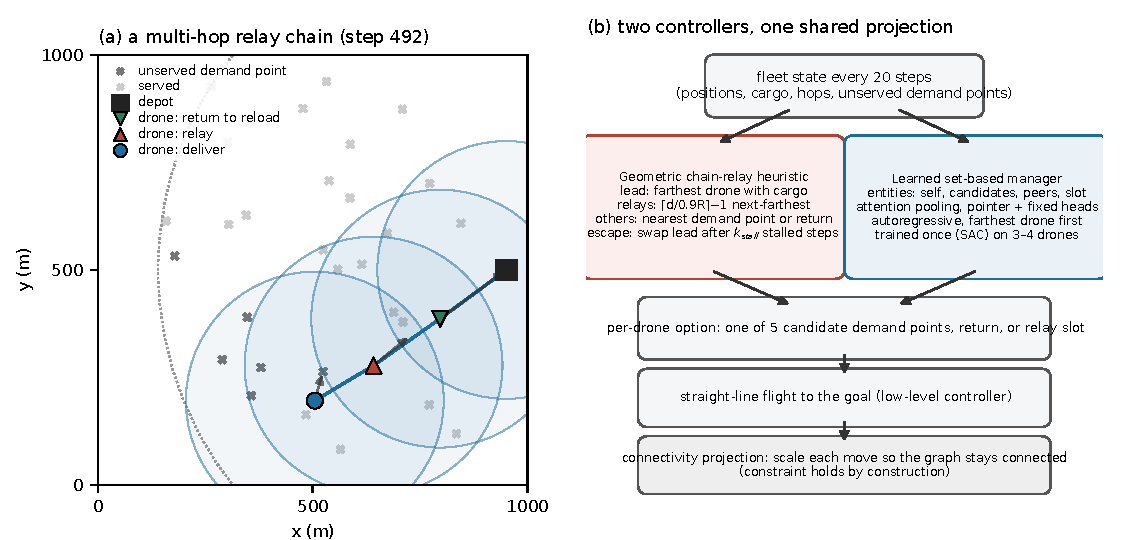
\includegraphics[width=\linewidth]{fig_overview_v5_26_10_17_15.pdf}
\caption{(a) An instance with three drones under the rule at step 499: the lead (blue
circle) heads for a far demand point, one drone relays on the segment to the depot (red
triangle), and one drone returns to the depot to reload (green triangle); shaded discs are
communication ranges and the dotted circle is the reachable region $0.9NR$. (b) The two
controllers emit the same per-drone options and share the straight-line low-level controller
and the connectivity projection.}
\label{fig:overview}
\end{figure*}

\subsection{Shared interface: options, relay slots, projection}
\label{sec:shared}

\paragraph{Decision points and options}
A decision point occurs every 20 steps, and additionally as soon as any drone's goal becomes
invalid: its demand point has been served by another drone, it has run out of cargo while heading
to a demand point, it has become full while heading to the depot, or its relay slot has
disappeared because the chain it belonged to shortened. At a decision point every drone receives
one of $K = 7$ options: one of its five \emph{candidate demand points}, which are the five
unserved demand points nearest to it; \emph{return} to the depot; or \emph{relay}. An option is
\emph{valid} for a drone only if it makes sense at that moment: a demand point option requires
cargo on board and an existing candidate, return requires the drone not to be full, and relay
requires a free relay slot (defined next) and at least one teammate that is not itself relaying.
Invalid options are masked for the learned policy and never produced by the rule; a drone
with no valid option returns to the depot.

\paragraph{Relay slots}
The environment, not the controller, decides where a relaying drone stands. For drone $i$ the
\emph{frontier} $f_i$ is the point farthest from the depot among the delivery goals of the other
drones and the current positions of the other non-relaying drones (if there is none, the farthest
unserved demand point). A chain to $f_i$ at distance $d$ needs $n = \min(\lceil d/(0.9R)
\rceil - 1,\ N-1)$ relay slots, placed on the segment from the depot to $f_i$ at the fractions
$1/(n+1), \dots, n/(n+1)$ of its length; the factor $0.9$ leaves slack so that a drone standing
slightly off its slot does not break the link. Drone $i$ takes the free slot nearest to it. A
drone whose slot disappears holds position until the next decision point. The controllers
therefore decide only \emph{whether} a drone relays; the slot follows from the fleet's geometry.

\paragraph{Low-level flight and connectivity projection}
Every step, each drone commands a displacement of length $v$ towards its goal (zero while it is
serving). Enforcing connectivity by a reward penalty would punish situations that no action can
prevent, for example a drone that is stationary while unloading and is stranded when a teammate
departs; connectivity is therefore enforced by projection. If the commanded positions keep
$G_t$ connected they are applied. Otherwise the projection repeatedly selects one moving drone,
scales its displacement down to the largest factor in $[0,1]$ under which the fleet is connected
(found by bisection with the other drones' current scalings fixed), and stops as soon as the
fleet is connected; at each round it selects the drone whose restriction leaves the most drones
connected and breaks ties at random, so that no single anchor drone is starved. The previous
positions are always connected, so zero scaling is a valid fallback and the constraint holds by
construction. A drone whose displacement is scaled below 10\% is \emph{stalled} for that step,
and a \emph{partial deadlock} is a step in which all but at most one of the moving drones are
stalled; the number of consecutive partial-deadlock steps, $\delta_t$, is what the rule's
recovery mechanism monitors. This projection scales a displacement along its own direction;
Section~\ref{sec:sensitivity} studies a variant that keeps the tangential component.

\subsection{Geometric chain-relay rule with deadlock recovery}
\label{sec:rule}

The rule is a deterministic rule evaluated at every decision point
(Procedure~1). It first gives every drone a default: a drone with cargo goes to
its nearest unserved demand point and a drone without cargo returns to the depot. It then selects
the \emph{lead}, the drone with cargo that is farthest from the depot, computes how many hops the
lead's target needs, and turns that many of the remaining drones, the farthest ones first, into
relays. The number of relays is adaptive and the relays are the drones already closest to where
the chain must stand, which is what makes the rule cheap: it costs $O(N \log N)$ per decision
and 0.05--0.12\,ms in our implementation.

\begin{figure}[t]
\footnotesize
\noindent\textbf{Procedure 1.} Geometric chain-relay rule with deadlock recovery, run at every
decision point. State kept between calls: remaining recovery length $e$ (initially 0) and recovery
count $m$ (initially 0); both reset at the start of an episode. Parameters:
$k_{\mathrm{stall}} = 120$, $h_{\mathrm{hold}} = 20$, mode $\in$ \{lead swap, retreat\}.
\begin{procsteps}
\item \textbf{Recovery trigger.} If the fleet has been in partial deadlock for
$\delta_t \ge k_{\mathrm{stall}}$ consecutive steps and $e = 0$, set $e \leftarrow
h_{\mathrm{hold}}$ and $m \leftarrow m + 1$.
\item \textbf{Default assignment.} For each drone $i$: if it has no cargo, option $\leftarrow$
return; else if it has no unserved candidate, option $\leftarrow$ relay; else option
$\leftarrow$ its nearest unserved demand point.
\item \textbf{Lead.} If no demand point is unserved, stop. Otherwise let $r_i = \|p_i - c\|$
and let the lead be the drone with cargo that maximises $r_i$ (if no drone has cargo, the drone
maximising $r_i$).
\item \textbf{Relay count.} Let $d = \max(r_{\mathrm{lead}}, \|d_{\mathrm{goal}} - c\|)$ where
$d_{\mathrm{goal}}$ is the lead's nearest unserved demand point, and
$n = \min(\max(1, \lceil d / (0.9R) \rceil) - 1,\ N - 1)$.
\item \textbf{Relay identity.} Sort the drones other than the lead by $r_i$ in decreasing order
and set the option of the first $n$ of them to relay.
\item \textbf{Recovery manoeuvre} (only if $e > 0$; then $e \leftarrow e - 1$). \emph{Lead swap}:
sort all drones by $r_i$ in decreasing order, let the new lead be the $\min(m, N-1)$-th drone of
that order (0-based), set the old lead's option to return and, if the new lead has cargo and an
unserved candidate, set its option to its nearest unserved demand point. \emph{Retreat}: set the
option of every drone except the lead to return.
\item Return the options; the environment converts them into goals and assigns relay slots.
\end{procsteps}
\label{proc:heur}
\end{figure}

\paragraph{Deadlock recovery}
Because the rule is deterministic, a geometry that stalls the fleet makes it re-issue the same
assignment at every decision point and the stall persists; without an recovery mechanism the rule
completes 62\% of standard instances. The recovery mechanism is a timed override. It \emph{starts}
at the first decision point at which the fleet has been in partial deadlock for at least
$k_{\mathrm{stall}}$ consecutive steps and no recovery is in progress. It \emph{lasts} for
$h_{\mathrm{hold}}$ decision points, that is, roughly $20\,h_{\mathrm{hold}}$ steps, fewer when
goals become invalid early; during these decision points the rule is evaluated as usual and then
overridden as in step~6. It \emph{ends} when the count $e$ reaches zero, after which the plain
rule resumes; if the deadlock persists it can start again at the next decision point. Two modes
are implemented. In \emph{lead swap} the current lead is sent back to the depot and the role of
lead passes to another drone; on the $m$-th recovery of an episode it passes to the $m$-th farthest
drone, so that repeated recoveries cycle through the fleet rather than swapping the same two drones.
In \emph{retreat} every drone except the lead returns towards the depot, which slackens the
chain. Section~\ref{sec:rq5-rule} selects the mode and the two parameters on tuning seeds;
lead swap with $k_{\mathrm{stall}} = 120$ and $h_{\mathrm{hold}} = 20$ is used in every comparison.

\subsection{Rollout lookahead on the rule}
\label{sec:lookahead}

The rule's weakest decision is the choice of target, which is made independently per drone and
myopically. The \emph{lookahead rule} keeps Procedure~1 as a base policy and replaces that choice by a
one-step rollout \cite{bertsekas1997rollout}: at a decision point it enumerates a set of candidate
assignments, simulates each to completion with the base rule, and commits to the assignment whose
simulated makespan is shortest. The candidate set is the rule's own assignment and, for each drone
with cargo and each of its three nearest unserved demand points that no teammate already targets,
the same assignment with that drone sent to that demand point. On the main configurations of
Section~\ref{sec:rq1} each candidate is also evaluated with a relay \emph{pre-positioning} toggle,
under which a relay that has reached its slot moves on to the slot of the next frontier; the
reference instances of Section~\ref{sec:rq2} omit the toggle. To bound the cost the lookahead is
evaluated every 100 steps or as soon as a goal becomes invalid, and the plain rule decides in
between. Rollouts are capped at 3{,}000 steps and an unfinished rollout is scored by its length plus
50 steps per unserved demand point. The lookahead needs the simulator and the instance, and costs
tens of seconds to minutes per instance rather than milliseconds per decision; it is a rule in the
sense that it involves no training and no search over a solution representation, and it is
included because a baseline that is cheap to build should be as strong as cheap methods allow.

\subsection{Search heuristics over visit orders and over task sequences}
\label{sec:search}

The rule decides myopically: at every decision point the lead goes to its nearest unserved demand
point. The third method keeps the rule's execution layer and replaces that choice by an offline
search over a solution representation, evaluated by simulation in the same continuous simulator,
so the objective needs no model of the dynamics and automatically respects the connectivity
constraint. We use two representations, the second containing the first.

\paragraph{Visit-order search}
A solution is a \emph{priority list} of demand points per drone. At a decision point a drone's
goal is the first demand point on its own list that is still unserved, or the depot if its list
is exhausted or it carries no cargo; relays and the deadlock recovery are assigned exactly as in
Procedure~1, steps 3--6. The initial solution is read off a run of the rule, by recording which
drone served which demand point in which order. Neighbours relocate one demand point to a random
position in a random list, swap two demand points between lists, or reverse a segment of one list.
The search is an iterated local search: first-improvement local search over the three neighbour
types, then a perturbation of three random moves applied to the best solution, accepted if it is no
worse, with three restarts of 400 simulations each.

\paragraph{Task-sequence search}
The visit-order search still leaves relaying to the rule's geometry: the rule decides how many
relays the lead needs and turns the farthest other drones into relays. The second representation
makes the relay assignment a search variable. A drone's list may now also contain tasks
\emph{relay until demand point $j$ is served} (by whichever drone serves it). A drone whose first
unfinished task is such a task relays on the slot of Section~\ref{sec:shared}, and forced relays
count towards the relays the lead needs, so the rule assigns only the remainder; a delivery that
ends a relay task triggers a decision point. A list without relay tasks therefore executes exactly
as in the visit-order search. Neighbours add four relay moves to the visit-order moves: insert a
relay task with a random trigger at a random position of a random list, delete one, move one within
its list, and change the demand point a relay waits for. When the deadlock recovery starts, the
relay tasks that are being executed are dropped. The search starts from the best visit-order
solution, so it can never be worse, and runs three restarts of 1{,}000 simulations each.

\paragraph{Evaluation}
The projection breaks ties at random (Section~\ref{sec:shared}), so one simulation of a solution
is a random variable. During the search every simulation of an instance uses the same tie-breaking
seed, which makes the objective deterministic; the reported value of a search is the median over
ten fresh tie-breaking seeds of its best solution, which removes any gain fitted to the search
seed. Both searches are offline: they need the instance in advance and spend minutes on it, so we
report them as quality references rather than as controllers.

\subsection{Hierarchical learned policy}
\label{sec:learned}

The learned controller is hierarchical (Figure~\ref{fig:arch}). The high level, a \emph{manager},
acts only at decision points and outputs one option per drone; the low level is the shared
straight-line flight of Section~\ref{sec:shared}, so the manager's choices are held for 20 steps
and the problem it solves is a semi-Markov decision process over options \cite{sutton1999}.
Only the manager is learned. Separating the levels has two consequences that the rest of the
design relies on: the manager sees the fleet at a coarse time scale at which a formation can be
held, and the low level, being a fixed rule, can be reasoned about and projected for connectivity
without learning.

\begin{figure*}[t]
\centering
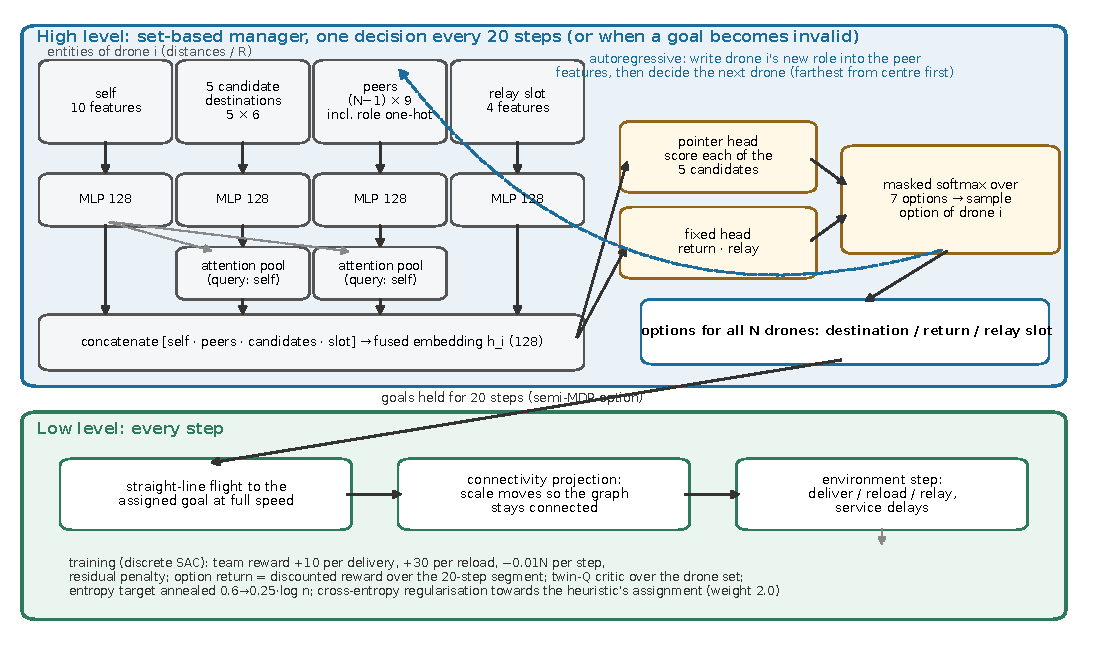
\includegraphics[width=\linewidth]{fig_arch_v5_26_10_19_10.pdf}
\caption{The hierarchical learned controller. High level: the set-based manager encodes each
drone from four kinds of entities, pools the peer and candidate sets with attention queried by
the drone's own embedding, and scores the five candidates with a pointer head and return/relay
with a fixed head; drones are decided one at a time, farthest from the depot first, and each
decision is written into the peer features seen by the next drone. Low level, every step:
straight-line flight to the assigned goal, the connectivity projection, and the environment step.
Options are held for 20 steps.}
\label{fig:arch}
\end{figure*}

\paragraph{Set-based encoder}
The manager encodes drone $i$ from four kinds of entities, all distances divided by $R$.
\emph{Own state}, 10 features: cargo fraction; distance to the depot; hop depth divided by 8;
fraction of demand points unserved; elapsed time divided by the budget; its realised-movement
ratio (an exponential average of achieved over commanded displacement); whether it could advance
one full step towards its goal alone without disconnecting the fleet; the fleet-wide
realised-movement ratio; service timer; and whether it is a cut vertex of $G_t$.
\emph{Candidate demand points}, five entities of 6 features: distance; the two components of the
unit direction vector; whether a teammate already targets it; its distance from the depot; and
the hops its chain requires, divided by 8. \emph{Peers}, $N-1$ entities of 9 features: distance;
the two components of the relative position vector; cargo fraction; hop depth divided by 8; and a
four-way one-hot of the peer's current goal kind (deliver, return, hold, relay). \emph{Relay
slot}, 4 features: distance; the two components of the unit direction vector; and the number of
slots in the current chain, divided by 8. Each entity type passes through a two-layer MLP of width 128. The drone's own embedding is
the query of two multi-head attention layers (4 heads) that pool the peer set and the candidate
set into one vector each; the four vectors are concatenated and fused by a further MLP into the
drone's embedding $h_i$. A \emph{pointer head} scores each candidate from $[h_i;\, e_{\mathrm{cand}}]$
and a \emph{fixed head} scores return and relay from $h_i$; the seven scores are masked and
normalised by a softmax. Nothing in the network depends on $N$ or $M$, which is why one set of
weights runs on fleets it never saw.

\paragraph{Autoregressive decision}
The $N$ options are not sampled independently. Drones are ordered by distance from the depot,
farthest first; the manager samples the first drone's option, writes its new role into the
role one-hot of the peer features that the remaining drones see, re-encodes, samples the next
drone, and so on (Procedure~2). A formation of one lead and $k$ relays arises
only by coincidence under independent sampling but can be composed deliberately under sequential
decisions; the cost is $N$ sequential network calls per decision point.

\begin{figure}[t]
\footnotesize
\noindent\textbf{Procedure 2.} Learned manager at a decision point (inference).
\begin{procsteps}
\item Build the entity observation of every drone from the fleet state; compute the validity mask
of the seven options for every drone (Section~\ref{sec:shared}).
\item Order the drones by distance from the depot, farthest first.
\item For each drone $i$ in that order: encode all entities with the current peer roles, compute
the seven masked logits of drone $i$, sample its option from the softmax (sampling, not argmax,
is the deployed inference), and write the chosen role (deliver, return or relay) into the peer
role one-hot of drone $i$ as seen by the drones not yet decided.
\item Return the $N$ options; the environment converts them into goals and assigns relay slots.
\end{procsteps}
\label{proc:learn}
\end{figure}

\paragraph{Training}
The manager is trained with discrete soft actor-critic \cite{haarnoja2018} on option
transitions. A transition stores the fleet observation at a decision point, the $N$ options,
the option return $\sum_{\tau} \gamma^{\tau} r_{\tau}$ accumulated over the steps until the next
decision point, the observation at that point, and the discount $\gamma^{\Delta t}$ with
$\gamma = 0.997$ per step. The team reward is $+10$ per delivery, $+30$ per reload, $-0.01N$
per step and a residual penalty of $-0.1N$ times the fraction of demand points still unserved.
A twin-Q critic with attention across the drone embeddings outputs per-drone action values whose
mean over drones is regressed on the option return; the actor minimises the standard expectation
form $\mathbb{E}_{a \sim \pi}[\alpha \log \pi(a) - Q(a)]$ per drone, with teacher forcing of
the autoregressive order. Three elements of the training configuration matter and are ablated in
Section~\ref{sec:rq5}. (i) The entropy target is annealed linearly from $0.6 \log
n_{\mathrm{valid}}$ to $0.25 \log n_{\mathrm{valid}}$ over the first 400 episodes: a high
target keeps the policy random enough to recovery deadlocks early in training, a low one lets it
hold a multi-step formation later. (ii) A cross-entropy term with weight 2.0 pulls the policy
towards the option the rule's assignment rule (Procedure~1, steps 2--5, without recovery)
would take, wherever that option is valid. (iii) Every training episode samples $N \in
\{3,4\}$, $M \in [20,80]$ and a random depot. Optimisation uses Adam at $3 \times 10^{-4}$,
batches of 256 transitions from a replay buffer of 60{,}000, one gradient step every 4
environment steps after a warm-up of 400 transitions, and Polyak averaging of the target critic
with $\tau = 0.005$. Checkpoints are scored every 50 episodes on 80 validation instances with a
3{,}000-step budget by $100f + 40(1 - \bar t/3000)$, where $f$ is the completion rate and $\bar
t$ the mean steps; training stops after eight evaluations without improvement or at 1{,}000
episodes. One run takes about 13 hours on a single RTX~5080 when four runs share the GPU.

% =====================================================================================
\section{Experimental Setup}
\label{sec:setup}

\paragraph{Instances and configurations}
Instances are generated from integer seeds; a seed, $N$, $M$ and the depot mode determine the
instance exactly, so two controllers can be run on identical instances. Evaluation seeds are
disjoint from the seeds used for training, for checkpoint selection and for tuning the rule.
We evaluate on the standard configuration ($N=4$, $M=50$, fixed depot) and on eight unseen
configurations with random depots: $N/M \in \{3/20, 3/30, 4/80, 5/50, 6/80, 8/150, 10/300, 12/400\}$.

\paragraph{Baselines}
Four learning-free baselines establish that the problem is not solved by naive assignment. All
use the shared interface of Section~\ref{sec:shared} and are evaluated at the same decision
points. \emph{Greedy, no relay} is step~2 of Procedure~1 alone: every drone with cargo flies to
its nearest unserved demand point and every empty drone returns; nobody ever relays, so the chain
is maintained only by the projection, which stalls the fleet. \emph{One (two) fixed relays}
assigns the first one (two) drones of the fleet to relay permanently and runs the greedy rule on
the others; the relay count is fixed in advance instead of adapting to the lead's distance.
\emph{Geometric rule, no recovery} is Procedure~1 without step~6. The lookahead rule of
Section~\ref{sec:lookahead} is run on the three main configurations and on the reference instances
of Section~\ref{sec:rq2}, and the two searches of Section~\ref{sec:search} on the reference
instances only. All learning-free controllers are deterministic except for the random
tie-breaking of the projection.

\paragraph{Reference model}
The continuous-position model of Section~\ref{sec:cont-model} is solved on five instances at
each of $M = 9, 10, 11, 12$ demand points with three drones and capacity $Q = 3$, so that at least
one reload is forced for $M \ge 10$, at $\kappa = 10$ and $\kappa = 5$, under the two-pass protocol
of that section; every demand point lies within $0.9NR$ of the depot and each instance has at
least four demand points beyond $R$, so relaying is unavoidable. Every plan the solver returns is
replayed in the continuous simulator. The controllers and the searches run on the same instances
in the continuous simulator with the same capacity, the learned policies as the median of 30
sampled runs per instance.

\paragraph{Paired protocol}
Averaging only the episodes each method completes favours the method that gives up on hard
instances, and a single long stall moves a 40-run mean by over 100 steps. All comparisons
between the two controllers are therefore \emph{paired}: both run on the same instance, the
difference is taken over instances both complete, and we report the median paired difference,
the win--loss count and a Wilcoxon signed-rank $p$-value. Inference samples from the policy;
deterministic argmax inference has the same median but a far heavier tail. The standard
configuration uses 480 runs (60 seeds, 8 repetitions, two independent measurement runs),
the $3/30$ and $5/50$ configurations 200 (40 seeds, 5 repetitions) and the remaining
configurations 80 (40 seeds, 2 repetitions). Repetitions differ because the projection's tie
breaking is random. We found 40 runs too few to support any claim about tails.

% =====================================================================================
\section{Results}
\label{sec:results}

\subsection{RQ1: Completion under the hard constraint}
\label{sec:rq1}

Connectivity was never violated in any training episode or evaluation run, as the projection
guarantees. Table~\ref{tab:completion} reports completion within the 10{,}000-step budget. The
learned policy completes every instance in every configuration. The rule with recovery
completes 98--100\%; its misses concentrate where drones are plentiful, where a long chain that
is not needed still gets stationed and stalls. Without the recovery mechanism the rule completes
61.7\% of standard instances, and the naive baselines complete almost none: the greedy assignment
pulls the fleet apart, and fixed relay counts are wrong for most instances because the number of
relays a demand point needs varies with its distance.

\paragraph{The lookahead rule}
Table~\ref{tab:look} adds the rollout lookahead of Section~\ref{sec:lookahead} on the same
instances. It completes every instance, including the three on which the rule stalls, and it is
faster than both online controllers on every configuration: 19\% faster than the rule and 21\%
faster than the learned policy's median at $3/30$, 25\% and 22\% at $4/50$, 30\% and 13\% at
$5/50$, winning 38 to 59 of 40 to 60 paired instances against each. It pays for this with one to
six minutes of simulation per instance, four to five orders of magnitude above the learned policy's
decision time, and with the need for a simulator of the instance at hand. Fleet size no longer
divides the space when this method is on the table: the question the rest of the paper answers is
what the two millisecond controllers achieve, and Section~\ref{sec:rq2} measures how far all of
them are from the optimum.

\begin{table}[t]
\centering
\caption{Mean makespan of the rule, the lookahead rule and the learned policy (per-instance
median of its paired runs) on the three main configurations in the continuous space, with the
number of completed instances or runs, wins--losses and Wilcoxon $p$ of the lookahead rule against
each, on instances all three complete, and its mean simulation time per instance.}
\label{tab:look}
\scriptsize
\setlength{\tabcolsep}{0.9pt}
\begin{tabular}{lrrrrrrrrr}
\toprule
config. & inst. & rule & lookahead & learned & \multicolumn{2}{c}{vs rule} & \multicolumn{2}{c}{vs learned} & time \\
\cmidrule(lr){6-7}\cmidrule(lr){8-9}
 & & & & & W--L & $p$ & W--L & $p$ & s/inst. \\
\midrule
3/30 & 40 & 600 (40/40) & 487 (40/40) & 620 (200/200) & 40--0 & $<10^{-4}$ & 39--1 & $<10^{-4}$ & 59 \\
4/50 & 60 & 926 (59/60) & 690 (60/60) & 880 (480/480) & 59--0 & $<10^{-4}$ & 59--0 & $<10^{-4}$ & 302 \\
5/50 & 40 & 669 (39/40) & 466 (40/40) & 536 (200/200) & 39--0 & $<10^{-4}$ & 38--1 & $<10^{-4}$ & 361 \\
\bottomrule
\end{tabular}%

\end{table}

\begin{table}[t]
\centering
\caption{Completion within the 10{,}000-step budget. Learning-free baselines on 120 (standard)
or 40 (unseen) runs; the two proposed controllers on the paired run counts of
Section~\ref{sec:setup}. $p$ is Fisher's exact test (two-sided) of each method's completion
count against the learned policy on the same configuration.}
\label{tab:completion}
\scriptsize
\setlength{\tabcolsep}{2.2pt}
\begin{tabular}{lrrrrrr}
\toprule
Method & $4/50$ std. & $p$ & $3/30$ & $p$ & $5/50$ & $p$ \\
\midrule
Greedy, no relay & 0\% & $<10^{-4}$ & 0\% & $<10^{-4}$ & 25\% & $<10^{-4}$ \\
One fixed relay & 0\% & $<10^{-4}$ & 2.5\% & $<10^{-4}$ & 40\% & $<10^{-4}$ \\
Two fixed relays & 3.3\% & $<10^{-4}$ & 52.5\% & $<10^{-4}$ & 65\% & $<10^{-4}$ \\
Rule, no recovery & 61.7\% & $<10^{-4}$ & 95\% & 0.027 & 92.5\% & 0.004 \\
Rule + recov.\ (prop.) & 473/480 & 0.015 & 200/200 & 1 & 191/200 & 0.004 \\
Learned (prop.) & \textbf{480/480} & --- & \textbf{200/200} & --- & \textbf{200/200} & --- \\
\midrule
 & $3/20$ & & $4/80$ & & $6/80$ & \\
Rule + recov.\ (prop.) & 80/80 & 1 & 80/80 & 1 & 79/80 & 1 \\
Learned (prop.) & \textbf{80/80} & & \textbf{80/80} & & \textbf{80/80} & \\
\midrule
 & $8/150$ & & $10/300$ & & $12/400$ & \\
Rule + recov.\ (prop.) & 80/80 & 1 & 80/80 & 1 & 80/80 & 1 \\
Learned (prop.) & \textbf{80/80} & & \textbf{80/80} & & \textbf{80/80} & \\
\bottomrule
\end{tabular}
\end{table}

\subsection{RQ2: Distance to the optimum of the reference model}
\label{sec:rq2}

\paragraph{Reference solutions}
Table~\ref{tab:cont} measures every method against the model of Section~\ref{sec:cont-model} on
twenty instances with three drones, capacity 3 and 9 to 12 demand points, each with four or more
demand points beyond the communication radius. With ten-step periods the model is solved to proven
optimality on four of the five instances with nine demand points and on two of five with ten, in
2--61 minutes; with eleven and twelve demand points the two passes close none of the gaps, which
remain between 7\% and 63\%, so there the table brackets each method's gap between the incumbent
and the dual bound. Halving the period to five steps doubles the number of periods and proves one
instance; on eight of the twenty instances it finds a plan 5--10 steps (4--8\%) shorter than the
ten-step plan and never more, and on the one instance proven at both resolutions the optimum falls
from 80 to 75 steps, so the ten-step discretisation costs a few percent at most. Every plan at
either resolution replays in the simulator with full delivery, no disconnection and zero tracking
error. The reference costs 111 solver-hours for seven proofs, and the second pass, although it
halves the horizon, proves only one instance that the first did not: the difficulty lies in the
combinatorics of where the relays stand, not in the horizon.

\paragraph{Result}
No method beats the model's incumbent on any instance, and the ordering of the online controllers
is the same in all eight rows. The lookahead rule is the closest of them, 19--53\% above the proven
optima and 15--39\% above the incumbents over the eight rows; the rule is 50--135\% above the
proven optima and 34--78\% above the incumbents; and the learned policy trained on 20--80 demand
points with capacity 5 is the farthest, 58--87\% above the proven optima and 45--92\% above the
incumbents, on instances with fewer demand points and a smaller capacity than any it was trained
on. The two offline searches lie between the lookahead rule and the model: the visit-order search
is 5--44\% and the task-sequence search 5--35\% above the proven optima, and 21--35\% and 12--30\%
above the incumbents over the rows.

\paragraph{The methods decompose the gap}
Averaged over all twenty instances against the ten-step incumbents, the rule is 55.3\% above the
model, the visit-order search 28.2\%, the lookahead rule 27.3\% and the task-sequence search
21.3\%. The visit-order search is faster than the rule on 18 of the 20 instances ($p = 2 \times
10^{-4}$, Wilcoxon), the task-sequence search faster than the visit-order search on 16 and slower
on one ($p = 3 \times 10^{-4}$) and faster than the lookahead rule on 14 of 20 ($p = 0.04$), while
the visit-order search and the lookahead rule are indistinguishable (8 against 11, $p = 0.52$).
Freeing the visit order thus removes 27 of the rule's 55 points, so the myopic choice of targets is
the largest single cost, and the lookahead rule, which frees the same choice online by simulation
instead of offline by search, removes 28. Freeing the relay assignment removes another 7: on 12 of
the 20 instances the best task sequence contains forced relays, that is, it overrides which drone
relays or until which delivery, the decision in which the learned policy and the rule differ
(Section~\ref{sec:rq3}). The remaining 21 points, an upper estimate where the model is not proven,
are what neither search can express through the shared interface: relays stand on the slot geometry
of Section~\ref{sec:shared} instead of moving towards where they are needed next, and services and
moves are not timed jointly across drones, as the model's plans are.

\paragraph{The learned policy on the reference distribution}
The transferred policy runs outside its training distribution here, so its gap mixes the quality of
its decisions with the cost of the transfer. We therefore trained the proposed recipe on the
reference instances' own distribution, three drones, 8--16 demand points, capacity 3 and random
depots, with two seeds and the standard budget, and report the seed with the higher holdout score
(Table~\ref{tab:cont}, ``in-dist.''). Both runs ended at the 1,000-episode cap with their best
holdout at episode 650. The reported seed (SQb) has a mean makespan of 274 against 272 for the
transferred policy and is 68\% above the incumbents on average, as the transferred policy is; the
two tie instance by instance (10--10, Wilcoxon $p=0.82$). The other seed (SQa) is slightly slower
(283, $p=0.07$ against the transferred policy). Both remain behind the rule (SQb wins 5 of 20,
$p=0.04$) and behind the lookahead on every instance. Training on the reference distribution
therefore does not change the reading: the transferred policy's gap is not a cost of the transfer
but of the decisions the policy makes, the same decisions it makes in distribution.

\paragraph{Teaching the policy the lookahead's choices}
Since the lookahead supplies what the policy lacks, we tried to train it in. In two runs of the
proposed recipe the regularisation target was the assignment the lookahead would choose at each
decision point instead of the rule's, computed online by simulating each candidate with the rule;
the target always lies in the policy's option set. Both runs are slower than the proposed policy
on all three main configurations, by 38 to 140 steps in paired median ($p \le 6 \times 10^{-4}$).
A diagnostic shows why. At 445 states along the proposed policy's own trajectories on $3/30$
where the two targets differ, the lookahead's choice shortens the remaining time by 33 steps on
average when the rule completes the episode but by 16 when the learned policy does, it is worse
than the rule's choice in 44\% of those states, and the two gains are uncorrelated ($r = 0.02$):
the target is right for a policy that will continue like the rule and close to a coin toss for
one that will not. Scoring the candidates with the policy itself as the continuation, as in
expert iteration, removes that mismatch but meets noise: from the same state one rollout of the
stochastic policy varies with a median standard deviation of 54 steps, more than the differences
to be detected. We therefore let the rule's lookahead propose one alternative and kept it as a
target, at five times the regularisation weight, only where six paired rollouts of the current
policy confirmed a gain of more than 20 steps ($t < -2$), which happened at about 7\% of the
decision points examined; elsewhere the rule's assignment stayed the target. Two such runs started
from the proposed weights, alongside two control runs that omit these targets. In one run of each
pair no checkpoint ever scored above the starting weights on validation; in the other pair the
targets have no measurable effect, the run and its control being indistinguishable on all three
configurations ($p \ge 0.39$), and continued training from the proposed weights is itself
harmful: both are 55--78 steps slower than the proposed policy ($p \le 10^{-4}$), whereas
re-evaluating the unchanged weights reproduces the proposed policy's values to within 17 steps.
Choosing options by the trained critic's action values instead of the actor does not help either
(1{,}022--1{,}208 steps on $3/30$ against 620). Within this framework the lookahead's gain is
available at decision time and not through training.

\paragraph{Distilling the lookahead}
A last attempt removes policy-gradient updates altogether: starting from the proposed weights, the
manager is trained by cross-entropy alone on the lookahead's choices, collected in the manner of
DAgger \cite{ross2011} on fleets of three and four drones with 20--80 demand points. The raw labels
are mostly noise: relabelling 472 states with a different tie-breaking seed reproduces the
lookahead's choice in only 67\% of them, and the median gain of a deviation from the rule's
assignment is four steps. We therefore score each candidate by two rollouts with common random
numbers, keep the lookahead's choice as the label only where it beats the rule's assignment by
more than ten steps, use the rule's assignment elsewhere, and stop training early on 10\% held-out
episodes; the first iteration, on the teacher's own states, outperformed later iterations that mix
in the student's. We report the result as an analysis, not as a third controller. The distilled
policy removes the three-drone deficit: on $3/30$ it is 34--50 steps faster than the proposed
policy in paired median over three training seeds ($p \le 0.002$ for each) and level with the rule
($-5$, $p = 0.48$); on $4/50$ it is 16--32 steps faster, significantly for one seed; on $5/50$ it
is 3--18 steps slower; and on larger fleets its median is indistinguishable from the proposed
policy's, with a heavier tail on $4/80$ and $6/80$ that the recovery override of
Section~\ref{sec:rq3} largely removes. On the reference instances it is 3--15\% faster than the
transferred policy and within 4\% of the rule in every row, and it does not approach the model,
remaining 55--96\% above the proven optima. Distillation therefore carries the part of the
lookahead that holds when the rule completes the rollouts, at three drones, but not the distance to
the teacher itself, which on $3/30$ finishes in 484 steps against 574 for the distilled policy.

\begin{table*}[t]
\centering
\caption{Continuous-position, time-discretised reference model (period $\kappa$ steps, three drones, capacity 3, five instances per row) against the controllers run in the continuous space. UB and LB are the mean incumbent and bound after the two solver passes (one hour cold, two hours warm-started with a tightened horizon); ``proven'' counts instances solved to optimality. Controller cells give the mean makespan over the five instances and, in parentheses, the mean gap in percent to the model's UB and, when a row is not fully proven, to its LB (the true gap lies between the two). Learned policies are medians of 30 sampled runs per instance: ``transfer'' is the policy trained on 20--80 demand points with capacity 5, ``in-dist.'' the policy trained on the same distribution as these instances (8--16 demand points, capacity 3), ``distilled'' the policy distilled from the lookahead rule (an analysis variant, not a proposed controller). The two offline searches of Section~\ref{sec:search} are scored by the median over ten tie-breaking seeds of the projection of their best plan. Every model plan replays in the continuous environment with full delivery, no disconnection and 0.0\,m tracking error.}
\label{tab:cont}
\scriptsize\setlength{\tabcolsep}{1.9pt}
\begin{tabular}{rrrrrlllllll}
\toprule
 & & & & & \multicolumn{2}{c}{Online, learning-free} & \multicolumn{2}{c}{Offline search} & \multicolumn{2}{c}{Learned (proposed)} & Analysis \\
\cmidrule(lr){6-7}\cmidrule(lr){8-9}\cmidrule(lr){10-11}\cmidrule(lr){12-12}
$\kappa$ & $M$ & proven & UB & LB & Rule & Lookahead & Visit order & Task seq. & Transfer & In-dist. & Distilled \\
\midrule
10 & 9 & 4/5 & 130 & 118 & 199 (+54/+68) & 172 (+33/+44) & 165 (+26/+37) & 156 (+20/+31) & 235 (+83/+99) & 234 (+80/+96) & 205 (+59/+73) \\
10 & 10 & 2/5 & 154 & 118 & 269 (+78/+126) & 195 (+30/+64) & 200 (+32/+68) & 188 (+24/+59) & 268 (+75/+125) & 258 (+69/+117) & 259 (+72/+118) \\
10 & 11 & 0/5 & 166 & 122 & 261 (+55/+111) & 220 (+32/+78) & 220 (+34/+79) & 212 (+29/+73) & 279 (+67/+127) & 288 (+74/+135) & 262 (+59/+114) \\
10 & 12 & 0/5 & 210 & 118 & 285 (+34/+139) & 242 (+15/+104) & 253 (+21/+113) & 235 (+12/+98) & 306 (+45/+158) & 315 (+49/+165) & 297 (+41/+150) \\
\midrule
5 & 9 & 1/5 & 124 & 84 & 199 (+62/+134) & 172 (+39/+102) & 165 (+32/+94) & 156 (+26/+83) & 235 (+92/+176) & 234 (+89/+175) & 205 (+67/+141) \\
5 & 10 & 0/5 & 154 & 84 & 269 (+78/+218) & 195 (+30/+130) & 200 (+32/+135) & 188 (+24/+122) & 268 (+75/+215) & 258 (+69/+204) & 259 (+72/+206) \\
5 & 11 & 0/5 & 165 & 85 & 261 (+56/+203) & 220 (+32/+155) & 220 (+35/+157) & 212 (+30/+148) & 279 (+68/+225) & 288 (+75/+236) & 262 (+60/+206) \\
5 & 12 & 0/5 & 208 & 86 & 285 (+35/+228) & 242 (+16/+180) & 253 (+22/+194) & 235 (+14/+173) & 306 (+47/+254) & 315 (+51/+265) & 297 (+43/+245) \\
\bottomrule
\end{tabular}
\end{table*}


\paragraph{Cost}
The searches and the lookahead buy their points with computation: the visit-order search takes
4.3 minutes per instance (1{,}200 simulations), the task-sequence search a further 9.9 minutes
(3{,}000 simulations) and the lookahead rule 4.7 seconds (1.2--8.8), all measured on a shared machine, against 0.05--0.12\,ms per decision for the rule and 2.7--7.4\,ms for the learned
policy (Table~\ref{tab:latency}); all three need the instance in advance or a simulator of it.
The model needs 2--61 minutes for each of its proofs at ten-step periods and leaves gaps of
7--63\% after three hours with eleven or twelve demand points.

\paragraph{Where the reference stops}
The model grows with the number of periods, which grows with the makespan, and its difficulty
grows with the number of ways to place the relays: with eleven and twelve demand points three
solver-hours close none of the gaps, and we did not push further. The reference therefore stops
two orders of magnitude below the instances the controllers are intended to run on; beyond it only
the comparison between methods of Section~\ref{sec:rq3} remains.

\subsection{RQ3: Comparative performance across operating conditions}
\label{sec:rq3}

\paragraph{Fleet size divides the configuration space}
Table~\ref{tab:paired} and Figure~\ref{fig:regime} give the paired comparison across the nine
configurations. With three drones the rule is faster by 39 and 30 steps in paired median with 20 and
30 demand points. With four drones the two controllers are statistically indistinguishable: on the standard configuration the
median paired difference over 480 runs is $+2$ steps with 234 wins against 239
($p = 0.52$), and on $4/80$ the learned policy is 38 steps faster. With five or more drones the
learned policy is faster, by 62 steps at five drones growing to 178 at ten and 76 at twelve
(70 wins against 10). The boundary therefore lies at four drones, and the advantage persists
beyond the largest fleet we measured, although the monotone growth stops between ten and twelve
(Section~\ref{sec:rq4} returns to this point). The split concerns the two millisecond
controllers; the lookahead rule of Table~\ref{tab:look} is faster than both on all three
configurations it was run on.
An earlier measurement against
the rule's pre-tuning recovery parameters gave the same picture ($+40$, $+0$, $-54$, $-170$ on
$3/30$, $4/50$, $5/50$ and $10/300$), so the boundary does not depend on the tuning.

\begin{table*}[t]
\centering
\caption{Paired comparison on identical instances. Positive differences mean the learned policy
is slower than the rule. $p$ from the Wilcoxon signed-rank test on both-completed pairs.}
\label{tab:paired}
\small
\begin{tabular}{lrrrrrr}
\toprule
$N/M$ & rollouts & complete h/l & median rule / learned & paired median & win--loss & $p$ \\
\midrule
3/20 & 80 & 80/80 & 364 / 420 & $+39$ & 22--58 & $<10^{-4}$ \\
3/30 & 200 & 200/200 & 572 / 618 & $+30$ & 81--119 & 3.4e-04 \\
4/50 (standard) & 480 & 473/480 & 878 / 878 & $+2$ & 234--239 & 0.521 \\
4/80 & 80 & 80/80 & 1,120 / 1,036 & $-38$ & 50--28 & 0.006 \\
5/50 & 200 & 191/200 & 588 / 534 & $-62$ & 147--44 & $<10^{-4}$ \\
6/80 & 80 & 79/80 & 737 / 614 & $-122$ & 72--7 & $<10^{-4}$ \\
8/150 & 80 & 80/80 & 916 / 722 & $-158$ & 75--5 & $<10^{-4}$ \\
10/300 & 80 & 80/80 & 1,216 / 1,052 & $-178$ & 69--11 & $<10^{-4}$ \\
12/400 & 80 & 80/80 & 1,199 / 1,108 & $-76$ & 70--10 & $<10^{-4}$ \\
\bottomrule
\end{tabular}%

\end{table*}

\begin{figure}[t]
\centering
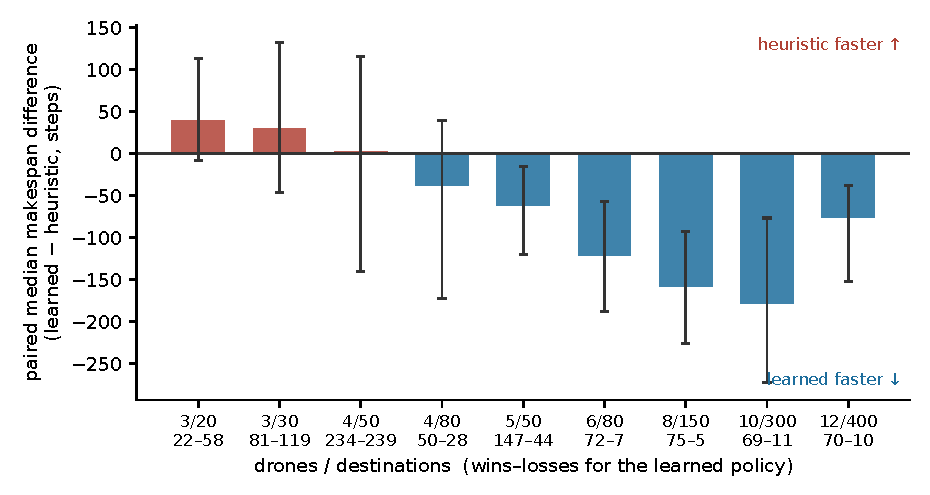
\includegraphics[width=\linewidth]{fig_regime_v5_26_10_17_15.pdf}
\caption{Paired median makespan difference (learned minus rule) by configuration, with the
interquartile range of the paired differences as error bars and the learned policy's wins--losses
under each label. Negative values favour the learned policy; the boundary lies at four drones.}
\label{fig:regime}
\end{figure}

Figure~\ref{fig:cdf} shows the full distributions on the three main configurations: with three
drones the rule's curve lies to the left, with four the curves coincide, and with five the
learned policy's curve lies to the left and reaches completion earlier.

\begin{figure*}[t]
\centering
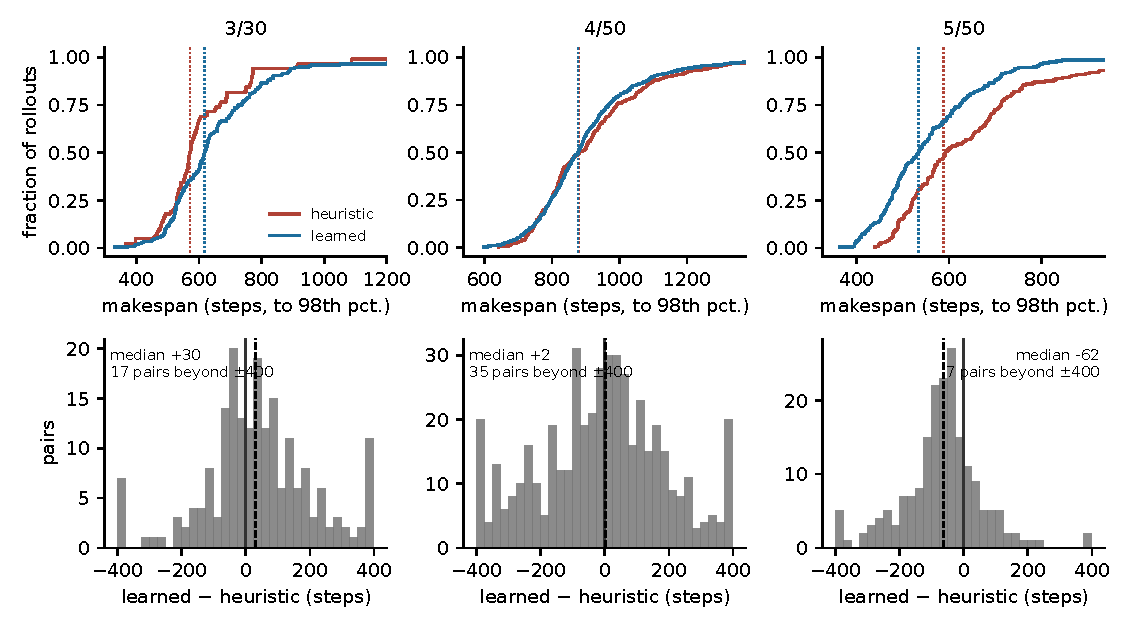
\includegraphics[width=\linewidth]{fig_cdf_v5_26_10_17_15.pdf}
\caption{Top: cumulative distribution of makespan on $3/30$, $4/50$ and $5/50$ (dotted lines
mark medians; axes cut at the 98th percentile). Bottom: distribution of the paired difference on
both-completed instances, clipped to $\pm400$ steps with the number of clipped pairs noted.}
\label{fig:cdf}
\end{figure*}

\paragraph{Tails follow the same split}
Where drones are scarce the learned policy's worst case is three to four times the rule's
(maximum 5{,}395 versus 1{,}447 steps on $3/30$); where they are plentiful it is lighter (1{,}101
versus 1{,}734 on $5/50$, 1{,}365 versus 1{,}753 on $10/300$). On the standard configuration over
480 runs against the pre-tuning rule the learned policy exceeded 1{,}500 steps five times
and the rule fourteen times.

\paragraph{Stabilising the tail}
That tail is a liability for a relief operation, where the worst case matters more than the
median, so we tried to remove it from both sides. On the \emph{training} side we trained four
further runs under the proposed configuration: two with the deadlock-recovery override inside the
rollout loop, so that the policy learns against the behaviour it will be deployed with, and two
with the entropy target annealed to $0.10 \log n_{\mathrm{valid}}$ instead of $0.25$, to make the
policy less random late in training. Neither worked. The lower entropy target doubled the spread
on $3/30$ (standard deviation 629 and 1{,}001 against 328 for the proposed policy, maxima of
6{,}283 and 9{,}049). Of the two runs with recovery in the loop, one matched the proposed policy
on $3/30$ ($+36$ against $+30$) and the other lost 110 steps of median, and evaluating the first
of them \emph{without} the override at inference restored the original spread (standard deviation
338, maximum 3{,}634), which shows that the training change did nothing and the override at
inference did the work.

On the \emph{inference} side, applying the rule's recovery step (Procedure~1, step~6) to the
proposed policy's options whenever the fleet has been in partial deadlock for
$k_{\mathrm{stall}}$ steps, with no retraining, removes the tail on every configuration
(Table~\ref{tab:stab}). The worst case falls from 4{,}614 to 1{,}210 steps on $3/30$ and from
3{,}061 to 1{,}436 on the standard configuration, the standard deviation falls by a third to a
half, and no run exceeds 1{,}500 steps where twelve did before. The median cost is confined to
the configuration where the learned policy was already behind: $+64$ instead of $+30$ on $3/30$,
while the standard configuration improves slightly ($-13$ against $+2$, both insignificant) and
$5/50$ is unchanged ($-54$ against $-62$). We therefore report the plain policy as the proposal,
because it is the faster one in the median, and recommend the override wherever the worst case is
what has to be guaranteed.

\begin{table*}[t]
\centering
\caption{Effect of the deadlock-recovery override applied to the proposed policy at inference,
without retraining. The paired median, wins--losses and $p$ are against the tuned rule on the
same instances; the standard deviation, 90th percentile, maximum and the count above 1{,}500 steps
describe the learned policy's own makespan distribution.}
\label{tab:stab}
\small
\begin{tabular}{llrrrrrrrr}
\toprule
config. & inference & runs & paired median & wins--losses & $p$ & s.d. & 90th pct. & max & $>$1{,}500 \\
\midrule
$3/30$ & proposed & 200 & $+30$ & 81--119 & 3.4e-04 & 328 & 837 & 4614 & 2 \\
 & + recovery & 200 & $+64$ & 66--134 & $<10^{-4}$ & 149 & 858 & 1210 & 0 \\
\addlinespace
$4/50$ & proposed & 480 & $+2$ & 234--239 & 0.521 & 208 & 1104 & 3061 & 7 \\
 & + recovery & 240 & $-13$ & 125--110 & 0.249 & 132 & 1052 & 1436 & 0 \\
\addlinespace
$5/50$ & proposed & 200 & $-62$ & 147--44 & $<10^{-4}$ & 125 & 712 & 1302 & 0 \\
 & + recovery & 200 & $-54$ & 145--44 & $<10^{-4}$ & 131 & 734 & 1075 & 0 \\
\bottomrule
\end{tabular}%

\end{table*}

\paragraph{Mechanism}
The two controllers differ in one decision. On $3/30$ the rule stations 1.39 relays on
average and the learned policy 0.78; the learned fleet therefore spends 27\% of drone-steps stalled
by the projection against 8\% for the rule. Overriding only the learned policy's relay
assignment with the rule's, at inference, recovers the full 44-step gap; matching only the
\emph{number} of relays recovers 14 steps of median but removes the tail (maximum from 4{,}904 to
1{,}083). The identity of the relaying drone drives the median and the count drives the tail. The
information needed to make the rule's choice is present in the learned policy's observation:
a two-layer classifier predicts the rule's relay assignment from the 41 observed features with
85\% accuracy, and behaviour cloning of the full rule reaches 95\% on relay decisions. When drones
are plentiful the opposite happens: the rule keeps stationing a chain that the geometry no
longer needs, while the learned policy exploits the slack and, with its sampled inference, recoveries
the stalls that the deterministic rule repeats; this is also where the rule loses its few
completions.

\paragraph{Why the relay-limited deficit resists policy-side fixes}
\label{sec:negative}
Table~\ref{tab:negative} lists eleven interventions, each trained with four or two seeds under
the same training configuration except for the stated change and evaluated with the same paired protocol, that
attempt to make the learned policy relay like the rule when drones are scarce. The variants
are, in the numbering of the table: (V1) the cross-entropy regularisation towards the rule is
weighted three times higher for drones whose rule option is relay; (V2) each drone on the
communication path of a delivering teammate receives an individual reward (2.0 or 6.0) at that
delivery and the critic is trained on per-drone returns; (V3) checkpoint selection scores half of
its validation instances on the $3/30$ configuration instead of only on $4/50$, eight seeds; (V4) as
V2 but zero-sum, the delivering drone losing what its relays gain; (V5) the critic is conditioned
on the teammates' chosen roles (a joint-action critic) with the teammates' next roles sampled
from the actor in the target; (V6) the autoregressive order is reversed to decide the drone
nearest the depot first; (V7) all goals are invalidated after 60 consecutive partial-deadlock
steps so that the manager re-decides, in training and evaluation; (V8) the mean over per-drone
action values in the critic is replaced by state-dependent monotone weights that sum to one with
a floor of one half; (V9) each drone's option is stored as its own single-agent transition,
chained inside a decision point with discount one, so that no decomposition of the team return is
needed; (V10) the manager is initialised by behaviour cloning of the rule on 40{,}000
decisions (92.5\% accuracy, 95\% on relay decisions) and then fine-tuned, with and without a
50-episode critic warm-up; (V11) a per-step penalty proportional to the estimated arrival time of
the bottleneck demand point, with the estimate divided by each drone's realised-movement ratio so
that blocked drones count as slow. None improves the $3/30$ median and several hurt the
configurations where the learned policy wins. The pattern is informative. Adding reward for
relaying turns the means into the end: the policy relays for its own sake and $5/50$ reverses from
$-54$ to $+60$. Every route to per-drone credit is blocked for a different reason: a joint-action
critic inherits the variance of a sampled teammate action in its target; a monotonic mixing
network either diverges when its weights are free or collapses to the mean when they are floored;
a sequential single-agent reformulation removes the decomposition but leaves an undiscounted
credit chain with no contraction. Initialising the policy by behaviour cloning of the rule, with
95\% relay accuracy, is erased within 400 episodes: once the actor is updated, relay usage falls to
the level of a randomly initialised policy within 50 episodes and stays there. A penalty on the
bottleneck demand point's estimated arrival makes the policy reduce the \emph{average} rather than
the maximum. We conclude that, within this policy structure and objective, under-relaying is the
learner's fixed point, not an artefact of credit, information or initialisation.

\begin{table*}[t]
\centering
\caption{Interventions that did not remove the relay-limited deficit, numbered as in the text.
Cells give the range over seeds of the paired median difference against the rule (positive:
learned slower) and, in parentheses, the number of seeds whose difference is significant at
$p<0.05$ (Wilcoxon signed-rank) over the number of seeds trained. The reference row is the
proposed policy against the tuned rule (Table~\ref{tab:paired}); the variant rows were
evaluated against the rule with its pre-tuning recovery parameters ($k_{\mathrm{stall}}=60$,
$h_{\mathrm{hold}}=40$), against which the proposed policy measured $+40$, $-54$ and $+0$, so
differences of a few tens of steps between the reference row and a variant row are not
meaningful.}
\label{tab:negative}
\scriptsize
\setlength{\tabcolsep}{3pt}
\begin{tabular}{llrrrl}
\toprule
\# & Intervention (what changed) & $3/30$ & $5/50$ & $4/50$ & Mechanism of failure \\
\midrule
--- & Proposed configuration (reference) & $+30$ (1/1) & $-62$ (1/1) & $+0$ (0/1) & --- \\
V1 & Relay-weighted rule regularisation ($\times 3$) & $+18$, $+58$ (1/2) & $-29$, $+13$ (0/2) & $+13$, $+41$ (1/2) & relay-specific regularisation harms \\
V2 & Per-drone relay credit (2.0 / 6.0) & $+36$ to $+82$ (4/4) & $+60$ to $+106$ (4/4) & $+39$ to $+131$ (4/4) & relaying becomes the goal \\
V3 & Checkpoint selection half on $3/30$ & $+37$ to $+105$ (8/8) & $-58$ to $-22$ (7/8) & $-37$ to $+108$ (3/8) & improves only the standard config. \\
V4 & Zero-sum credit redistribution & $+91$, $+126$ (2/2) & $+98$, $+172$ (2/2) & $+146$, $+180$ (2/2) & same, larger \\
V5 & Joint-action critic & $+71$ to $+124$ (4/4) & $-46$ to $-16$ (3/4) & $+8$ to $+100$ (2/4) & target variance from sampled teammates \\
V6 & Nearest-first decision order & $+46$, $+100$ (2/2) & $-43$, $-38$ (2/2) & $+4$, $+106$ (1/2) & order is not the cause \\
V7 & Re-decision after 60 stalled steps & $+82$, $+95$ (2/2) & $-38$, $-34$ (2/2) & $+17$, $+55$ (0/2) & irregular option lengths \\
V8 & Monotone mixing critic (floor 0.5) & $+54$ to $+230$ (4/4) & $-28$ to $+38$ (2/4) & $+55$ to $+258$ (4/4) & divergence vs.\ credit on one axis \\
V9 & Sequential single-agent credit & $+81$ to $+213$ (4/4) & $+8$ to $+27$ (2/4) & $+62$ to $+170$ (4/4) & no contraction within a decision \\
V10 & Behaviour-cloning initialisation ($\pm$ warm-up) & $+6$ to $+69$ (3/4) & $-42$ to $-20$ (3/4) & $-16$ to $+40$ (0/4) & erased within 400 episodes \\
V11 & Bottleneck-arrival penalty (0.15 / 0.25) & $+85$ to $+144$ (4/4) & $-32$ to $+13$ (2/4) & $+7$ to $+156$ (3/4) & reduces the mean, not the maximum \\
\bottomrule
\end{tabular}%

\end{table*}

\paragraph{Sensitivity to the connectivity enforcement model}
\label{sec:sensitivity}
The projection of Section~\ref{sec:shared} scales a blocked displacement along its own
direction, so a drone pulling on the chain effectively stops. We implemented an alternative that
clamps the target position to the nearest point of the communication disc around the binding
neighbour, which removes only the outward component and keeps the tangential one (a drone can
still circle at constant range). Both controllers use the same projection in each comparison, and
connectivity is still never violated. These measurements predate the rule tuning of Section~\ref{sec:rq5-rule} and use
$k_{\mathrm{stall}}=60$, $h_{\mathrm{hold}}=40$ for both projections, so they are internally
consistent. Evaluating the same learned weights under the sliding projection without retraining
reduces the $3/30$ deficit from $+40$ to $+21$; retraining four
seeds under it gives $+15$ to $+48$ (mean $+28$) and lowers the learned fleet's stall ratio from
0.27 to 0.17--0.22, with completion still 100\%. The rule gains little with three drones
(median 570 to 571) but gains more than the learned policy with four (866 to 812 against 879 to
850), so the standard-configuration equality becomes $+26$ in its favour. We therefore keep the radial
projection as the primary model and report this as a sensitivity result: about half of the
three-drone deficit is a property of how the constraint is enforced rather than of the learner.

\paragraph{Communication radius}
Both controllers were run without retraining at $R = 250$\,m and $R = 350$\,m
(Table~\ref{tab:range}, Figure~\ref{fig:range}); the learned policy normalises distances by $R$,
and the instance generator rescales the reachable region $0.9NR$ with $R$, so both controllers see
the same instances at each radius. Completion transfers: the learned policy completes every
instance at both radii, while the rule loses 18 of 200 instances on $5/50$ at the shorter
radius. Speed shows two effects. The first is the regime shift seen with fleet size: at
$R=250$\,m a demand point needs more hops, the fleet is effectively scarcer, and every
configuration moves towards the rule ($+77$ on $3/30$, $+68$ on $4/50$, and the $5/50$
advantage shrinks to an insignificant $-16$ ($p=0.33$)); at $R=350$\,m the fleet is effectively more
plentiful and the learned policy is faster already with four drones ($-40$ on $4/50$). The second
is a training-radius effect: on $3/30$ and $5/50$ the learned policy's margin is best at the
radius it was trained on and worse on both sides ($+30$ at 300\,m against $+77$ and $+52$;
$-62$ against $-16$ and $-42$), so the normalisation by $R$ transfers completion but not the full
speed. The regime variable is therefore the chain demand, the hops a demand point needs relative
to the drones available, rather than the fleet size alone, and a deployment at a radius far from
the training radius should retrain or at least re-evaluate the boundary.

\begin{figure}[t]
\centering
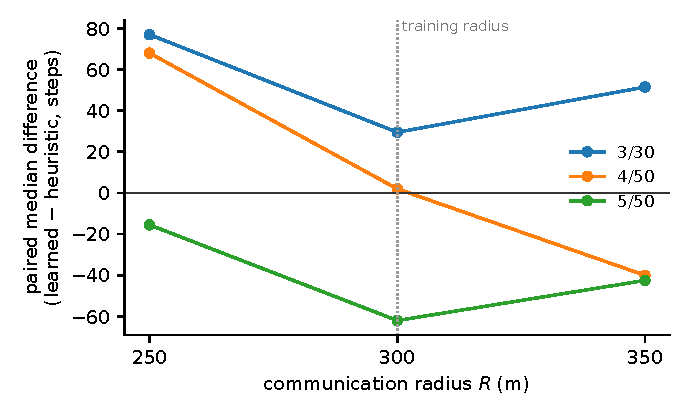
\includegraphics[width=\linewidth]{fig_range_v5_26_10_17_15.pdf}
\caption{Transfer to other communication radii without retraining, one panel per
configuration. Bars are the paired median difference (learned $-$ rule, steps): a bar above
zero (red) means the rule was faster, below zero (blue) the learned policy; whiskers are the
interquartile range of the paired differences, the label at each bar is the learned policy's
wins--losses, and the completions (rule/learned) are printed under the radius. The shaded
column is the training radius. Reading left to right within a panel: a shorter radius moves every
configuration towards the rule, and on $3/30$ and $5/50$ the learned policy's margin is best
at the radius it was trained on.}
\label{fig:range}
\end{figure}

\begin{table*}[t]
\centering
\caption{Transfer to other communication radii without retraining. Cells give completions
(rule/learned) and the paired median difference with win--loss and $p$; $R=300$\,m is the
training radius.}
\label{tab:range}
\small
\begin{tabular}{lrrr}
\toprule
$N/M$ & $R=250$\,m & $R=300$\,m & $R=350$\,m \\
\midrule
3/30 & --- & 200/200 \,/\, $+40$ (73--127, $<10^{-4}$) & --- \\
4/50 & --- & 473/480 \,/\, $+0$ (236--236, 0.885) & --- \\
5/50 & --- & 190/200 \,/\, $-54$ (141--45, $<10^{-4}$) & --- \\
\bottomrule
\end{tabular}%

\end{table*}

\subsection{RQ4: Upward transfer of the learned policy}
\label{sec:rq4}

The learned policy never saw more than four drones or more than 80 demand points in training,
yet it completes every instance with 5 to 12 drones and 50 to 400 demand points and is faster
than the rule on all of them. Two properties carry this. The set-based encoder has no
parameter that depends on $N$ or $M$, so larger fleets are simply larger sets; and training
samples the fleet size and depot afresh every episode. Table~\ref{tab:gen} separates the two by
running the ablation policy that was trained on the fixed $4/50$ configuration alone (no
configuration randomisation) on the same large-fleet instances without retraining. That policy
also completes every instance from 5 to 10 drones, so completion generalises through the
architecture alone; but it is slower than the randomised policy on every configuration (no significant difference
from the rule at $5/50$ against $-62$, and $-51$ to $-174$ against $-122$ to $-178$ beyond),
so speed on large fleets is learned from the variety of small ones. The same ablation loses 114--296
steps on $3/30$ (Table~\ref{tab:ablation}), so randomisation is what makes the small-fleet side
usable at all. Both policies were trained with at most four drones; the hop-depth and slot
features are normalised by a constant of eight, so fleets of ten and twelve drones also take the
encoder outside its training range of feature values, and the policy still completes them.

\begin{table*}[t]
\centering
\caption{Transfer to fleets larger than any seen in training, without retraining. Cells
give the learned policy's completions, the paired median difference against the rule
(negative: learned faster), and in parentheses the learned policy's wins--losses and the
Wilcoxon signed-rank $p$.
The proposed policy is trained on $N \in \{3,4\}$ with random depots; the comparison policy is
the ablation trained on the fixed $4/50$ configuration only (two seeds).}
\label{tab:gen}
\small
\begin{tabular}{lrrr}
\toprule
$N/M$ & trained on $N\in\{3,4\}$, $M\in[20,80]$ & trained on $4/50$ only, seed 1 & seed 2 \\
\midrule
5/50 & 200/200 \,/\, $-62$ (147--44, $<10^{-4}$) & 80/80 \,/\, $+7$ (35--39, 0.840) & 80/80 \,/\, $+44$ (28--50, 0.002) \\
6/80 & 80/80 \,/\, $-122$ (72--7, $<10^{-4}$) & 80/80 \,/\, $-56$ (57--20, $<10^{-4}$) & 80/80 \,/\, $-51$ (51--27, 0.010) \\
8/150 & 80/80 \,/\, $-158$ (75--5, $<10^{-4}$) & 80/80 \,/\, $-129$ (68--11, $<10^{-4}$) & 80/80 \,/\, $-110$ (60--20, $<10^{-4}$) \\
10/300 & 80/80 \,/\, $-178$ (69--11, $<10^{-4}$) & 80/80 \,/\, $-152$ (69--11, $<10^{-4}$) & 80/80 \,/\, $-174$ (68--12, $<10^{-4}$) \\
\bottomrule
\end{tabular}%

\end{table*}

\paragraph{Where the transfer weakens}
We have not isolated the cause of the narrowing at $12/400$ and offer three conjectures. First,
both controllers maintain a single chain to one lead, so with twelve drones most of the fleet is
delivering near the depot regardless of the controller and the decisions that differ between
them concern a shrinking share of the work. Second, with 400 demand points a drone's five
candidates are all close to it, so the choice among them matters less and the learned policy's
advantage, which lies in choosing targets and relays jointly, has less to act on. Third, the
manager's hop-depth and slot features are normalised by a constant of eight and exceed one for
larger fleets, and twelve sequential autoregressive decisions compound sampling noise; both take
the policy farther from its training distribution. Which of these dominates would require fleets
beyond twelve drones to settle.

\subsection{RQ5: Are the components necessary?}
\label{sec:rq5}

\paragraph{Rule}
\label{sec:rq5-rule}
Table~\ref{tab:heur-ablation} grids $k_{\mathrm{stall}} \in \{30,60,90,120\}$,
$h_{\mathrm{hold}} \in \{20,40,80\}$ and the two recovery modes, plus no recovery, on $3/30$,
$4/50$ and $5/50$ with 40 tuning seeds each, and ranks settings by total completions first and
the sum of median makespans second; this criterion was fixed before the measurement. The recovery
mechanism is necessary: without it the rule completes 25--26 of 40 standard instances (two
measurements). The mode matters more than the timing: every lead-swap setting completes 117--120
of 120 instances, while retreat settings complete 101--117 because slackening the chain does not
change the assignment that caused the stall. Within the lead-swap family the differences are not
statistically meaningful: in a second measurement of the grid, reported in the table together with
a paired Wilcoxon test of every setting against the selected one on the same 40 instances, no
setting differs from the selected one at $p<0.05$ on any configuration (all $p \ge 0.09$), and
one other setting ($30/40$) also completes all 120 with a median sum 13 steps lower, which is
tie-breaking noise. The selected setting ($k_{\mathrm{stall}}=120$, $h_{\mathrm{hold}}=20$)
was fixed from the first measurement and is used throughout. The adaptive relay count is necessary as well: fixing one or two
relays completes 0--65\% (Table~\ref{tab:completion}).

\begin{table*}[t]
\centering
\caption{Rule ablation on tuning seeds disjoint from the evaluation seeds (40 instances per
configuration). Cells give completed instances, the median makespan over completed instances and,
in parentheses, the $p$-value of a Wilcoxon signed-rank test of that setting against the selected
setting (bold) on the instances both completed; the last column sums completions over the three
configurations.}
\label{tab:heur-ablation}
\small
\begin{tabular}{llrrrr}
\toprule
mode & $k_{\mathrm{stall}}$ / $h_{\mathrm{hold}}$ & $3/30$ & $4/50$ & $5/50$ & completions \\
\midrule
none & --- & 39/40 \,/\, 559 (0.228) & 25/40 \,/\, 817 (0.258) & 38/40 \,/\, 602 (0.093) & 102/120 \\
lead swap & 30 / 20 & 40/40 \,/\, 557 (0.121) & 39/40 \,/\, 853 (0.130) & 40/40 \,/\, 625 (0.928) & 119/120 \\
lead swap & 30 / 40 & 40/40 \,/\, 562 (0.673) & 40/40 \,/\, 867 (0.775) & 40/40 \,/\, 606 (0.247) & 120/120 \\
lead swap & 30 / 80 & 40/40 \,/\, 567 (0.158) & 39/40 \,/\, 844 (0.754) & 39/40 \,/\, 614 (0.404) & 118/120 \\
lead swap & 60 / 20 & 40/40 \,/\, 557 (0.599) & 39/40 \,/\, 849 (0.780) & 40/40 \,/\, 600 (0.791) & 119/120 \\
lead swap & 60 / 40 & 40/40 \,/\, 554 (0.497) & 39/40 \,/\, 852 (0.807) & 40/40 \,/\, 625 (0.944) & 119/120 \\
lead swap & 60 / 80 & 40/40 \,/\, 556 (0.359) & 39/40 \,/\, 863 (0.788) & 39/40 \,/\, 632 (0.675) & 118/120 \\
lead swap & 90 / 20 & 40/40 \,/\, 566 (0.206) & 39/40 \,/\, 871 (0.908) & 40/40 \,/\, 599 (0.375) & 119/120 \\
lead swap & 90 / 40 & 40/40 \,/\, 559 (0.473) & 40/40 \,/\, 856 (0.674) & 37/40 \,/\, 634 (0.844) & 117/120 \\
lead swap & 90 / 80 & 40/40 \,/\, 563 (0.786) & 39/40 \,/\, 858 (0.149) & 39/40 \,/\, 629 (0.615) & 118/120 \\
\textbf{lead swap} & \textbf{120 / 20} & 40/40 \,/\, 561 & 40/40 \,/\, 867 & 40/40 \,/\, 620 & \textbf{120/120} \\
lead swap & 120 / 40 & 40/40 \,/\, 557 (0.757) & 39/40 \,/\, 878 (0.685) & 40/40 \,/\, 624 (0.979) & 119/120 \\
lead swap & 120 / 80 & 40/40 \,/\, 562 (0.687) & 38/40 \,/\, 829 (0.546) & 39/40 \,/\, 626 (0.850) & 117/120 \\
retreat & 30 / 20 & 37/40 \,/\, 559 (0.350) & 35/40 \,/\, 836 (0.185) & 40/40 \,/\, 632 (0.528) & 112/120 \\
retreat & 30 / 40 & 39/40 \,/\, 556 (0.079) & 29/40 \,/\, 832 (0.284) & 39/40 \,/\, 621 (0.157) & 107/120 \\
retreat & 30 / 80 & 38/40 \,/\, 561 (0.754) & 26/40 \,/\, 804 (0.443) & 37/40 \,/\, 584 (0.368) & 101/120 \\
retreat & 60 / 20 & 39/40 \,/\, 556 (0.866) & 38/40 \,/\, 847 (0.215) & 38/40 \,/\, 603 (0.759) & 115/120 \\
retreat & 60 / 40 & 39/40 \,/\, 559 (0.875) & 39/40 \,/\, 823 (0.485) & 39/40 \,/\, 624 (0.459) & 117/120 \\
retreat & 60 / 80 & 39/40 \,/\, 563 (0.991) & 26/40 \,/\, 795 (0.236) & 40/40 \,/\, 635 (0.490) & 105/120 \\
retreat & 90 / 20 & 39/40 \,/\, 566 (0.512) & 38/40 \,/\, 822 (0.058) & 40/40 \,/\, 642 (0.773) & 117/120 \\
retreat & 90 / 40 & 39/40 \,/\, 566 (0.180) & 39/40 \,/\, 852 (0.634) & 39/40 \,/\, 618 (0.615) & 117/120 \\
retreat & 90 / 80 & 39/40 \,/\, 562 (0.665) & 36/40 \,/\, 830 (0.578) & 37/40 \,/\, 598 (0.354) & 112/120 \\
retreat & 120 / 20 & 39/40 \,/\, 556 (0.645) & 37/40 \,/\, 863 (0.327) & 38/40 \,/\, 614 (0.460) & 114/120 \\
retreat & 120 / 40 & 39/40 \,/\, 560 (0.757) & 37/40 \,/\, 831 (0.451) & 38/40 \,/\, 628 (0.602) & 114/120 \\
retreat & 120 / 80 & 39/40 \,/\, 561 (0.191) & 38/40 \,/\, 854 (0.815) & 37/40 \,/\, 627 (0.308) & 114/120 \\
\bottomrule
\end{tabular}%

\end{table*}

\paragraph{Learned policy}
Table~\ref{tab:ablation} removes one element at a time, retrains two seeds with the same budget,
and runs each ablated policy on the same instances as the proposed policy (the first 120, 80 and
80 paired runs of Section~\ref{sec:rq3}); cells give the median of the per-instance makespan
difference and a Wilcoxon signed-rank $p$, per seed. Rule regularisation and entropy-target
annealing are necessary everywhere: removing either costs 52--189 steps on every configuration
and seed at $p<10^{-4}$. Configuration randomisation is necessary off the training distribution:
removing it is neutral on the standard configuration ($-19$ and $-34$, $p \ge 0.12$), on which
the ablated policy was trained, but costs 114--296 steps on $3/30$ and 53--76 on $5/50$.
Autoregressive decisions help on every configuration by 32--88 steps ($p \le 0.007$). The
residual penalty is neutral: no seed on any configuration differs from the proposed policy at
$p<0.05$. A manager with a fixed-size MLP encoder instead of the set encoder, trained in an
earlier version on the standard configuration only, completed 38\% of standard instances and could
not be run on other fleet sizes at all.

\begin{table*}[t]
\centering
\caption{Ablation of the learned policy. Each cell gives, for two independently trained seeds,
the median per-instance makespan difference between the ablated policy and the proposed policy on
the same instances (positive: the removed element was needed) and the Wilcoxon signed-rank $p$.}
\label{tab:ablation}
\footnotesize
\begin{tabular}{lrrr}
\toprule
Removed component & $4/50$ (120 runs) & $3/30$ (80) & $5/50$ (80) \\
\midrule
Rule regularisation & $+121$ ($<10^{-4}$) / $+189$ ($<10^{-4}$) & $+171$ ($<10^{-4}$) / $+160$ ($<10^{-4}$) & $+52$ ($<10^{-4}$) / $+152$ ($<10^{-4}$) \\
Configuration randomisation & $-19$ (0.260) / $-34$ (0.119) & $+114$ ($<10^{-4}$) / $+296$ ($<10^{-4}$) & $+53$ (2.7e-04) / $+76$ ($<10^{-4}$) \\
Entropy target annealing & $+136$ ($<10^{-4}$) / $+138$ ($<10^{-4}$) & $+138$ ($<10^{-4}$) / $+130$ ($<10^{-4}$) & $+58$ ($<10^{-4}$) / $+76$ ($<10^{-4}$) \\
Autoregressive decisions & $+32$ (0.007) / $+84$ ($<10^{-4}$) & $+88$ (3.2e-04) / $+56$ (0.002) & $+42$ (2.7e-04) / $+60$ (9.1e-04) \\
Residual penalty & $-4$ (0.746) / $-32$ (0.204) & $+16$ (0.625) / $-28$ (0.291) & $+24$ (0.120) / $+12$ (0.374) \\
\bottomrule
\end{tabular}%

\end{table*}

\subsection{Inference cost}
\label{sec:cost}

Table~\ref{tab:latency} gives the latency of one manager decision on a CPU. The rule costs
0.05--0.12\,ms; the learned policy 1.3--2.5\,ms without autoregression and 2.7--7.4\,ms with it,
growing linearly with the fleet because each drone is a sequential network call. Over a 900-step
episode the learned policy's cumulative decision time is 0.16\,s. The lookahead rule spends 59,
302 and 361 seconds per instance on $3/30$, $4/50$ and $5/50$ (Table~\ref{tab:look}), that is,
0.1--0.5 seconds of simulation per decision point. The reference model needs 2--61 minutes per
proof with nine and ten demand points and three hours do not suffice with eleven or twelve.

\begin{table*}[t]
\centering
\caption{Latency of one manager decision (milliseconds, CPU) and the cumulative decision time of
a 900-step episode.}
\label{tab:latency}
\small
\begin{tabular}{lrrrrr}
\toprule
Controller & $N=3$ & $N=4$ & $N=6$ & $N=8$ & 900 steps \\
\midrule
Geometric rule + recovery & 0.05 & 0.08 & 0.10 & 0.12 & 0.003\,s \\
Learned, independent decisions & 1.27 & 1.52 & 1.94 & 2.45 & 0.069\,s \\
Learned, autoregressive (proposed) & 2.70 & 3.52 & 5.32 & 7.35 & 0.158\,s \\
\bottomrule
\end{tabular}
\end{table*}

% =====================================================================================
\section{Discussion}
\label{sec:discussion}

\paragraph{Deployment}
If a few minutes of simulation per instance are affordable, the lookahead rule is the controller
to run: it completes everything we gave it and is 13--30\% faster than either millisecond
controller on every configuration measured. When decisions must be made in milliseconds, the
two online controllers are complementary and the boundary is sharp, so a fleet operator can
choose by fleet size: the rule with three drones, the learned policy with five or more, where it
is both faster and more reliable; with four the two are statistically indistinguishable in speed
and the learned policy completes more. All of them keep the fleet connected by construction.

\paragraph{What the negative results mean}
Eleven interventions that change how the learner is credited, informed, initialised or rewarded leave
the relay-limited deficit in place, and a change to the environment's enforcement model removes
half of it. The deficit is therefore best understood as an interaction between the learner's
fixed point under this objective and the geometry of the constraint, not as a shortcoming that
more training or a better critic would fix. The same reading applies to the gap to the optimum:
training the policy towards the lookahead's choices fails twice, once because the target assumes
the rule's continuation and once because the verified signal is sparse and continued training
costs more than it adds; distilling refined lookahead labels without policy-gradient updates
removes the three-drone deficit but leaves the distilled policy where the rule is, far from its
teacher; training on the reference instances' own distribution leaves the policy where the transferred one is; and a one-step lookahead at decision time
removes much of the rule's gap. What the learner lacks is the non-myopic target choice that simulation supplies, and
in this framework simulation has to supply it when the decision is made. For a practitioner the
actionable consequence is the one above: pick the controller by the latency budget first and by
regime second.

\paragraph{Limitations}
The learned policy was trained at a single communication radius; it transfers to radii of 250 and
350\,m in completion but its speed ranking against the rule shifts with the radius
(Section~\ref{sec:rq3}), and radii outside this range were not tested. The environment is planar, ignores
wind, battery and collisions, and uses a disc communication model; real links are not discs. The
reference optimum is that of a time-discretised model: halving its period shortens the best plan
by at most 4--8\% on our instances, so the measured gaps understate the true ones by about that
much, the reference covers three drones and at most twelve demand points, and beyond ten demand
points only incumbents with a remaining optimality gap are available. The two searches execute
through the rule's slot geometry and the same option interface as the controllers, so they bound
what that interface can achieve under search rather than the problem's optimum. The lookahead rule extends to large fleets, at a cost that grows with the episode
length and the fleet. The
rule's novelty lies in the recovery mechanism and the adaptive relay count rather than in the
chain geometry itself.

\paragraph{Methodological notes}
Four practices mattered for the conclusions. Completed-episode averages favour the controller that
gives up, so comparisons must be paired. Forty runs cannot support claims about tails; several
of our own interim conclusions reversed when the sample grew. A pre-check that uses a different
metric from the final judgement will pass interventions that the final judgement rejects. And
checkpoint selection on a validation set with one sampled run per instance cannot see a
degradation of 55--78 steps that a paired evaluation on other instances detects at
$p < 10^{-4}$; validation scores of runs started from identical weights spread over two points,
as much as separates a good checkpoint from a poor one.

% =====================================================================================
\section{Conclusion}
\label{sec:conclusion}

We proposed two controllers for connectivity-constrained drone delivery, a geometric chain-relay
rule with deadlock recovery and a fleet-size-agnostic learned policy, both acting through a
projection that keeps the fleet connected at every step. Under a paired protocol across fleets of
three to twelve drones the learned policy completes every instance and is faster by 38 to 178
steps once more than four drones are available, although it was trained on three and four, while the rule is faster by 30--39 steps with
three. The relay-limited deficit is one decision, which drone relays; it resists eleven policy-side
interventions and halves when the enforcement model is changed. Against a continuous-position,
time-discretised reference model that is solved to proven optimality on six of twenty small
instances and bounded on the rest, the rule is 50--135\% and the learned policy 58--87\% above the
proven optima, a one-step rollout lookahead on the rule 19--53\%, and over all twenty instances
offline searches over visit orders and over task sequences are 28\% and 21\% above the model's
plans, against 55\% for the rule. The
headroom lies first in choosing targets and then in assigning relays, and simulation supplies the
first part: the lookahead rule is also 13--30\% faster than both online controllers on the main
configurations, at minutes per instance, whereas training the policy towards the lookahead's
choices does not reduce its median, and distilling the lookahead removes the three-drone deficit
without approaching the teacher. The case for the learned policy is therefore its millisecond
latency and its transfer to large fleets, where neither the reference model nor the searches
reach. The natural next step is a policy whose output is a team assignment rather than a set of
per-drone options, so that the relay identity becomes a coordinate a critic can value directly.

\section*{Acknowledgements}
\pending{To be added.}

\section*{Data and code availability}
Code, trained weights, instance generators and the paired-comparison records are available at
\url{https://github.com/koptimizer/relay_drone_network}.

\bibliographystyle{elsarticle-num}
\bibliography{paper_v5_26_10_17_15}

\end{document}
